\documentclass[11pt]{article}
\usepackage[scaled=0.92]{helvet}
\usepackage{geometry}
\geometry{letterpaper,tmargin=1in,bmargin=1in,lmargin=1in,rmargin=1in}
\usepackage[parfill]{parskip} % Activate to begin paragraphs with an empty line rather than an indent %\usepackage{graphicx}
\usepackage{amsmath,amssymb, mathrsfs,  mathtools, dsfont}
\usepackage{tabularx}
\usepackage{tikz-cd}
\usepackage[font=footnotesize,labelfont=bf]{caption}
\usepackage{graphicx}
\usepackage{xcolor}
%\usepackage[linkbordercolor ={1 1 1} ]{hyperref}
%\usepackage[sf]{titlesec}
\usepackage{natbib}
\usepackage{../../Tianpei_Report}

%\usepackage{appendix}
%\usepackage{algorithm}
%\usepackage{algorithmic}

%\renewcommand{\algorithmicrequire}{\textbf{Input:}}
%\renewcommand{\algorithmicensure}{\textbf{Output:}}



\begin{document}
\title{Lecture 2: Topological Space and Continuous Functions}
\author{ Tianpei Xie}
\date{Nov. 7th., 2022}
\maketitle
\tableofcontents
\newpage
\section{Topological Spaces}
\subsection{Definitions}
\begin{itemize}
\item 
\begin{definition} \citep{munkres2000topology}\\
Let $X$ be a set. \underline{\emph{A \textbf{topology}}} on $X$ is \emph{a collection} $\mathscr{T}$ of \emph{subsets} of X, called \emph{\textbf{open subsets}}, satisfying
\begin{enumerate}
\item $X$ and $\emptyset$ are \emph{open}.
\item The \emph{\textbf{union}} of \emph{\textbf{any family}} of open subsets is open.
\item The \emph{\textbf{intersection}} of \emph{any \textbf{finite} family} of open subsets is open.
\end{enumerate}
A pair $(X, \mathscr{T})$ consisting of a set $X$ together with a topology $\mathscr{T}$ on $X$ is called \emph{\textbf{a topological space}}.
\end{definition}

\item \begin{example}(\emph{\textbf{Discrete and Trivial Topology}})\\
If $X$ is any set, \emph{the collection of \textbf{all subsets}} of $X$ is a \emph{topology} on $X$; it is called \underline{\emph{\textbf{the discrete topology}}}. 

The collection consisting of \emph{$X$ and $0$ only} is also a \emph{topology} on X; we shall call it \emph{the \textbf{indiscrete topology}}, or \underline{\emph{\textbf{the trivial topology}}}.
\end{example}

\item \begin{example} (\emph{\textbf{The Finite Complement Topology}})\\
Let $X$ be a set; let $\srT_{f}$ be the collection of all subsets $U$ of $X$ such that \emph{$X \setminus U$ either is \textbf{finite} or is \textbf{all of} $X$}. Then $\srT_f$ is a topology on $X$, called \underline{\emph{\textbf{the finite complement topology}}}. 

Both $X$ and $\emptyset$ are in $\srT_{f}$, since $X \setminus X = \emptyset$ is finite and $X \setminus \emptyset$ is all of $X$. If $\{U_{\alpha}\}$ is
an \emph{indexed family of nonempty elements} of $\srT_{f}$, to show that $\cup_{\alpha}U_{\alpha}$ is in $\srT_{c}$, we compute
\begin{align*}
X \setminus \bigcup_{\alpha} U_{\alpha} &= \bigcap_{\alpha} (X \setminus U_{\alpha})
\end{align*}
The latter set is \emph{finite} because each set $X \setminus U_{\alpha}$ is \emph{finite}. If $U_1 \xdotx{,} U_n$ are nonempty elements of $\srT_f$, to show that $\cap_i U_i$ is in $\srT_f$, we compute
\begin{align*}
X - \bigcap_{i=1}^{n} U_i &= \bigcup_{i=1}^{n}(X - U_i)
\end{align*}
The latter set is a \emph{finite union of finite sets} and, therefore, \emph{finite}. \qed
\end{example}

\item \begin{definition} (\emph{\textbf{Comparable Topologies on the Same Set}})\\
Suppose that $\srT$ and $\srT'$ are two topologies on a given set $X$. If $\srT' \supseteq \srT$, we say that $\srT'$  is \underline{\emph{\textbf{finer}} (or \emph{\textbf{stronger}})} than $\srT$; if $\srT'$ \emph{\textbf{properly} contains} $\srT$ , we say that $\srT'$ is \underline{\emph{\textbf{strictly finer}}} than $\srT$. 

We also say that $\srT$ is \underline{\emph{\textbf{coarser}} (or \emph{\textbf{weaker}})} than $\srT'$, or \underline{\emph{\textbf{strictly coarser}}}, in these two respective situations. We say $\srT$ is \emph{\textbf{comparable}} with  $\srT'$ if either $\srT' \subseteq \srT$ or $\srT \subseteq \srT'$.
\end{definition}

\item \begin{remark}
\emph{\textbf{Topology}} of a set $X$ defines \emph{\textbf{all local information}} we know regarding a set. For each point  $x \in X$, it specifies what do we mean by a ``\emph{\textbf{neighborhood}}" $U$ of $x$. Thus properties that relies on the \emph{\textbf{local characteristic}} of the space  likely depend on the topology of the space. Examples include \emph{the continuity} of function, \emph{the convergence properties} of sequence and \emph{differential properties} of function. 
\end{remark}

\end{itemize}

\subsection{Basis for a Topology}
\begin{itemize}
\begin{figure}
\begin{minipage}[t]{1\linewidth}
  \centering
  \centerline{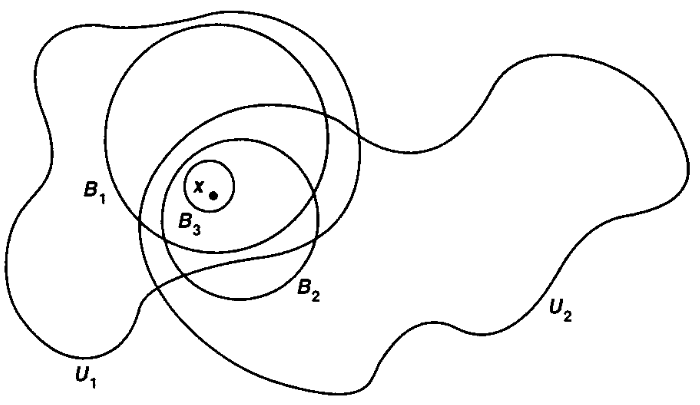
\includegraphics[scale = 0.4]{topology_basis.png}}
\end{minipage}
\caption{\footnotesize{\textbf{The basis of a topology \citep{munkres2000topology}}}}
\label{fig: topology_basis}
\end{figure}

\item \begin{definition}
Suppose $X$ is a topological space. A collection $\mathscr{B}$ of open subsets of $X$ is said to be \emph{\textbf{a basis}} for \emph{the topology of $X$} (plural: \emph{\textbf{bases}}) if every open subset of $X$ is the \emph{union of some collection of elements} of $\mathscr{B}$.

More generally, suppose $X$ is merely a set, and $\mathscr{B}$ is a collection of \emph{subsets} of $X$ satisfying the following conditions:
\begin{enumerate}
\item $X = \bigcup_{B \in \mathscr{B}}B$.
\item If $B_1, B_2 \in \mathscr{B}$ and $x \in B_1 \cap B_2$, then there exists $B_3 \in \mathscr{B}$ such that $x \in B_3 \subseteq B_1 \cap B2$.
\end{enumerate}
Then \emph{the collection of \textbf{all unions} of elements of $\mathscr{B}$} is a \emph{topology} $\srT$ on X, called \emph{\textbf{the topology $\srT$ \underline{generated by $\mathscr{B}$}}}, and $\mathscr{B}$ is a \underline{\emph{\textbf{basis}} for this \emph{topology}}.
\end{definition}

\item \begin{remark} (\emph{\textbf{Basis Element in Each Neighborhood}})\\
By definition, a subset $U$ of X is said to be \emph{\textbf{open}} in $X$ (that is, to be an element of $\srT$) if for each $x \in U$, there exists a \emph{\textbf{basis element}} $B \in \srB$ such that $x \in B \subset U$. Note that each basis element is itself an element of $\srT$.
\end{remark}

\item \begin{lemma}
Let $X$ be a set; let $\srB$ be a basis for a topology $\srT$ on $X$. Then $\srT$ equals the collection of \textbf{all unions} of elements of $\srB$.
\end{lemma}

\item \begin{remark}
This lemma states that every open set $U$ in X can be expressed as a \emph{union} of \emph{basis elements}. This expression for $U$ is \emph{\textbf{not}}, however, \emph{\textbf{unique}}.
\end{remark}

\item \begin{lemma} (\textbf{Obtaining Basis from Given Topology}). \citep{munkres2000topology}\\
Let $X$ be a topological space. Suppose that $\srC$ is a collection of open sets of $X$ such that for each open set $U$ of $X$ and each $x$ in $U$, there is an element $C$ of $\srC$ such that $x \in C \subset U$. Then $C$ is a basis for the topology of $X$.
\end{lemma}

\item \begin{lemma} (\textbf{Topology Comparison via Bases}). \citep{munkres2000topology}\\
Let $\srB$ and $\srB'$ be bases for the topologies $\srT$ and $\srT'$, respectively, on $X$. Then the following are equivalent:
\begin{enumerate}
\item  $\srT'$ is \textbf{finer} than $\srT$.
\item For each $x \in X$ and each basis element $B \in \srB$ containing $x$, there is a basis element $B' \in \srB'$ such that $x \in B' \subset B$.
\end{enumerate}
\end{lemma}

\item \begin{remark}
The \emph{\textbf{basis element}} of \emph{\textbf{finer} topology} are always \emph{\textbf{smaller}} than \emph{the basis element} of \emph{coaser topology} so the finer basis element should be included in coaser basis element.
\end{remark}

\item \begin{example} (\emph{\textbf{Topology} in $\bR$})\\
If $\srB$ is the collection of all \emph{\textbf{open intervals}} in the real line,
\begin{align*}
(a,b) = \{x: a < x < b\},
\end{align*}
the topology generated by $\srB$ is called \underline{\emph{\textbf{the standard topology}}} on the real line. Whenever we consider $\bR$, we shall suppose it is given this topology unless we specifically state otherwise.

If $\srB'$ is the collection of all \emph{half-open} intervals of the form
\begin{align*}
[a,b) = \{x: a \le  x < b\},
\end{align*} where $a < b$, the topology generated by $\srB'$ is called \underline{\emph{\textbf{the lower limit topology} on $\bR$}}. When $\bR$ is given \emph{the lower limit topology}, we denote it by $\bR_{\ell}$.

Finally let $K$ denote \emph{the set of all numbers of the form} $1/n$, for $n \in \bZ_{+}$,and let $\srB''$ be the collection of \emph{all open intervals} $(a,b)$, along with \emph{all sets of the form $(a,b) \setminus K$}. The topology generated by $\srB"$ will be called \underline{\emph{\textbf{the K-topology} on $\bR$}}. When $\bR$ is given this topology, we denote $\bR_{K}$

\begin{lemma}
The topologies of $\bR_{\ell}$ and $\bR_{K}$ are \textbf{strictly finer} than \textbf{the standard topology} on $\bR$, but are not comparable with one another.
\end{lemma}
\end{example}

\item \begin{definition}(\emph{\textbf{Subbasis}})\\
\underline{\emph{\textbf{A subbasis}} $\srS$ for a \emph{topology} on $X$} is a collection of subsets of $X$ whose union equals $X$. The topology generated by the \emph{subbasis} $\srS$ is defined to be the  collection $\srT$ of \emph{\textbf{all unions} of \textbf{finite intersections} of elements of $\srS$}.
\end{definition}

\item \begin{remark}(\textbf{\emph{Basis from Subbasis}})\\
For a \emph{subbasis} $\srS$, the collection $\srB$ of \emph{\textbf{all finite intersections}} of elements of $\srS$ is a \emph{\textbf{basis}},
\end{remark}
\end{itemize}

\subsection{The Order Topology}
\begin{itemize}
\item \begin{example}(\emph{\textbf{Order Topology}})\\
If $X$ is \emph{\textbf{a simply ordered set}}, there is a \emph{\textbf{standard topology}} for $X$, defined using the order relation. It is called \underline{\emph{\textbf{the order topology}}}. The order topology is generated by \emph{\textbf{intervals}}.
\end{example}

\item \begin{definition} (\emph{\textbf{Intervals based on Simple Order Relation}})\\
Suppose that $X$ is a set having \emph{a simple order relation} $<$. Given elements $a$ and $b$ of $X$ such that $a < b$, there are \emph{four subsets} of X that are called \emph{\textbf{the intervals}} determined by $a$ and $b$. They are the following :
\begin{align*}
(a,b) = \{x: a < x < b\},\\
(a,b] = \{x: a < x \le b\},\\
[a,b) = \{x: a \le x < b\},\\
[a, b] = \{x: a \le x \le b\}.
\end{align*}
A set of the \emph{first} type is called \underline{\textit{\textbf{an open interval}}} in $X$, a set of the \emph{last} type is called \underline{\textit{\textbf{a closed interval}}} in $X$, and sets of \emph{the second and third} types are called \underline{\textit{\textbf{half-open intervals}}}.
\end{definition}

\item \begin{definition}
Let $X$ be a set with a \emph{\textbf{simple order relation}}; assume $X$ has more than one element. Let $\srB$ be the collection of all sets of the following types:
\begin{enumerate}
\item \emph{\textbf{All open intervals}} $(a, b)$ in $X$.
\item \emph{\textbf{All intervals of the form $[a_0,b)$}}, where $a_0$ is the \emph{\textbf{smallest element}} (if any) of $X$.
\item \emph{\textbf{All intervals of the form $(a, b_0]$}}, where $b_0$ is the \emph{\textbf{largest element}} (if any) of $X$.
\end{enumerate}
The collection $\srB$ is a basis for a topology on $X$, which is called \underline{\emph{\textbf{the order topology}}}.
\end{definition}

\item \begin{definition}(\emph{\textbf{Rays}})\\
If $X$ is an ordered set, and $a$ is an element of $X$, there are four subsets of $X$ that are called \emph{\textbf{\underline{the rays}} determined by $a$}. They are the following:
\begin{align*}
(a, +\infty) = \{x:  x > a\},\\
(-\infty, a) = \{x:  x < a\},\\
[a, +\infty) = \{x: x \ge a\},\\
(-\infty, a]= \{x: x \le a\}.
\end{align*}
Sets of the first two types are called \emph{\textbf{open rays}}, and sets of the last two types are called \emph{\textbf{closed rays}}.
\end{definition}

\item \begin{remark}
The \emph{\textbf{open rays}} in $X$ are \emph{open sets} in \emph{\textbf{the order topology}}. In fact, \emph{\textbf{the open rays} form a \underline{\textbf{subbasis}} for \textbf{the order topology} on $X$}.
\end{remark}
\end{itemize}

\subsection{The Product Topology}
\begin{itemize}
\item \begin{definition} (\emph{\textbf{Product Topology}})\\
Let $X$ and $Y$ be topological spaces. \underline{\emph{\textbf{The product topology}}} on $X \times Y$ is the topology having as basis the collection $\srB$ of all sets of the form $U \times V$, where $U$ is an open subset of $X$ and $V$ is an open subset of $Y$.
\end{definition}

\begin{figure}
\begin{minipage}[t]{0.5\linewidth}
  \centering
  \centerline{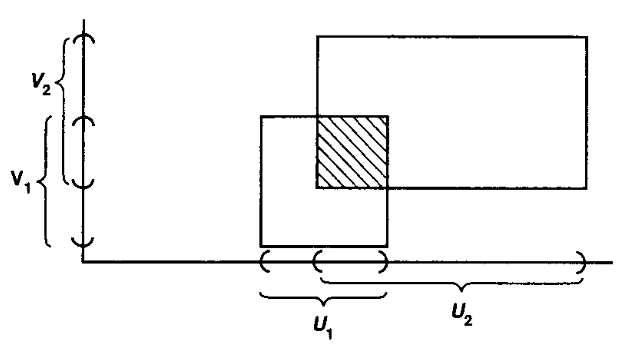
\includegraphics[scale = 0.34]{basis_product_topology.png}}
\end{minipage}
\begin{minipage}[t]{0.5\linewidth}
  \centering
  \centerline{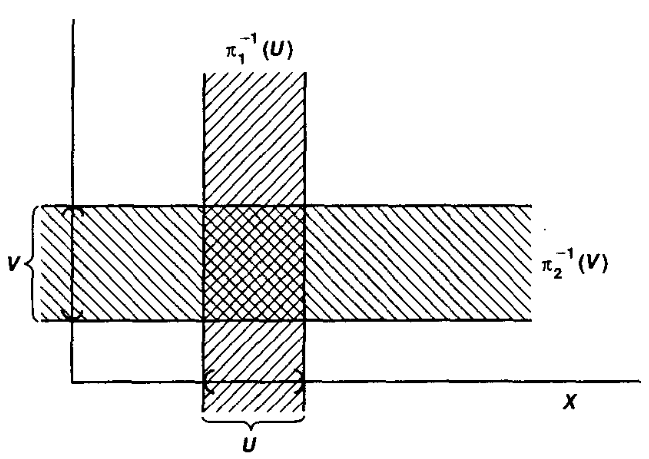
\includegraphics[scale = 0.34]{subbasis_product_topology.png}}
\end{minipage}
\caption{\footnotesize{\textbf{(Left) The basis of a product topology (Right) The subbasis of a product topology \citep{munkres2000topology}}}}
\label{fig: basis_product_topology}
\end{figure}


\item \begin{proposition} (\textbf{Basis of Product Topology})\\
If $\srB$ is a \textbf{basis} for the topology of $X$ and $\srC$ is a \textbf{basis} for the topology of $Y$, then the collection
\begin{align*}
\srD = \set{B \times C: B \in \srB, \text{ and } C \in \srC}
\end{align*}
is a \textbf{basis} for the topology of $X \times Y$.
\end{proposition}

\item It is sometimes useful to express the product topology in terms of a \emph{subbasis}. To do this, we first define certain functions called \emph{projections}.
\begin{definition}
Let $\pi_1 : X \times Y \rightarrow X$ be defined by the equation
\begin{align*}
\pi_1 (x, y) = x;
\end{align*}
$\pi_2 : X \times Y \rightarrow Y$ he defined by the equation
\begin{align*}
\pi_2 (x, y) = y.
\end{align*}
The maps $\pi_1$ and $\pi_2$ are called \emph{the \textbf{projections} of $X \times Y$ \textbf{onto} its \textbf{first} and \textbf{second} factors}, respectively.
\end{definition} 

\item \begin{remark}
Both $\pi_1$ and $\pi_2$ are \emph{\textbf{surjective}}. If $U$ is an \emph{\textbf{open}} subset of $X$, then the set $\pi_1^{-1}(U)$ is precisely the set $U \times Y$, which
is \emph{\textbf{open}} in $X \times Y$. 

Similarly, if $V$ is \emph{\textbf{open}} in $Y$, then $\pi_2^{-1}(V) = X \times V$ which is also \emph{\textbf{open}} in $X \times Y$.
\end{remark}

\item \begin{proposition}  (\textbf{Subbasis of Product Topology})\\
The collection
\begin{align*}
\srS = \set{\pi_1^{-1}(U): U\text{ open in }X} \cup \set{\pi_2^{-1}(V): V\text{ open in }Y}
\end{align*}
is a \emph{\textbf{subbasis}} for \textbf{the product topology} on $X \times Y$.
\end{proposition}
\end{itemize}

\subsection{The Subspace Topology}
\begin{itemize}
\item \begin{definition}
If $(X, \srT)$ is a topological space and $S \subseteq X$ is an arbitrary subset, we define \emph{\textbf{the \underline{subspace topology}}} on $S$ (sometimes called \emph{the \textbf{relative topology}}) as
\begin{align*}
\srT_{S} &= \set{S\cap U: U \in \srT}
\end{align*} 
That is, a subset $U \subseteq S$ to be \emph{open} in $S$ \emph{if and only} if there exists an \emph{open} subset $V \subseteq X$ such that $U = V \cap S$.  Any subset of $X$ endowed with \emph{the subspace topology} is said to be \emph{\textbf{a subspace of $X$}}.
\end{definition}

\item \begin{lemma} (\textbf{Basis of Subspace Topology})\\
If $\srB$ is a basis for the topology of $X$ then the collection
\begin{align*}
\srB_{S} = \set{B \cap S:  B \in \srB}
\end{align*}
is a \textbf{basis}  for the subspace topology on $S \subset X$.
\end{lemma}

\item \begin{remark} (\emph{\textbf{Open Relative to Which Set ?}})\\
When dealing with a space $X$ and a \emph{subspace} $Y$, one needs to be careful when one uses the term ``\emph{open set}". Does one mean \emph{an element of \textbf{the topology of $Y$}} or \emph{an element of \textbf{the topology of $X$}} ? We make the following definition : If $Y$ is a subspace of $X$, we say that \emph{\textbf{a set $U$ is open in $Y$}} (or \emph{open \textbf{relative} to $Y$}) if it belongs to the topology of $Y$; this implies in particular that it is a subset of $Y$. We say that \emph{\textbf{$U$ is open in $X$}} if it belongs to the topology of $X$.
\end{remark}

\item \begin{lemma} (\textbf{Open Subspace})\\
Let $Y$ be a subspace of $X$. If $U$ is open in $Y$ and $Y$ is open in $X$, then $U$ is open in $X$.
\end{lemma}

\item \begin{proposition} (\textbf{Product of Subspace Equal to Subspace of Product}) \citep{munkres2000topology}\\
If $A$ is a subspace of $X$ and $B$ is a subspace of $Y$, then \textbf{the product topology} on $A \times B$ is the same as the topology $A \times B$ inherits as a \textbf{subspace} of $X \times Y$.
\end{proposition}

\item \begin{remark} (\emph{\textbf{Subspace Topology  $\neq$ Order Topology on Subspace}})\\
Now let $X$ be an ordered set in \emph{the order topology}, and let $Y$ be a subset of $X$. The order relation on $X$, when restricted to $Y$, makes $Y$ into an ordered set. \emph{However}, \emph{the resulting order topology on $Y$ \textbf{need not be the same} as the topology that $Y$ inherits as a subspace of $X$}.

\begin{figure}
\begin{minipage}[t]{1\linewidth}
  \centering
  \centerline{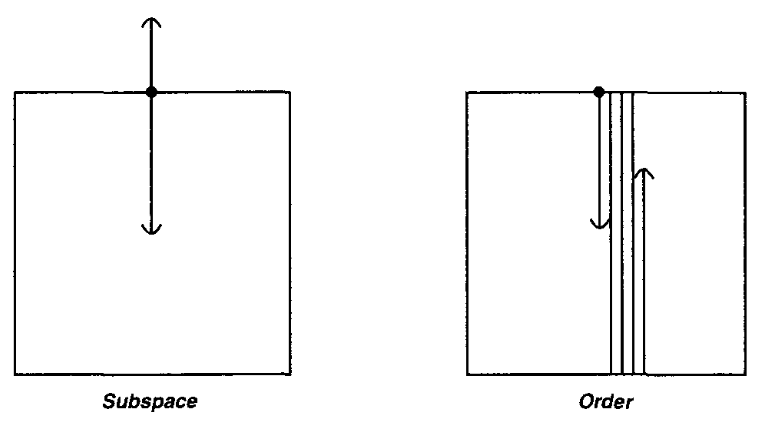
\includegraphics[scale = 0.4]{subspace_order_topology.png}}
\end{minipage}
\caption{\footnotesize{\textbf{(Left) The subspace topology inherited from amient space (Right) The order topology on subspace \citep{munkres2000topology}}}}
\label{fig: subspace_order_topology}
\end{figure}

Let $I= [0, 1]$. The \emph{dictionary order} on $I \times I$ is just \emph{the restriction to $I \times I$ of the dictionary order} on the plane $\bR \times \bR$. However, \emph{\textbf{the dictionary order topology}} on $I \times I$ is \emph{\textbf{not the same}} as \emph{\textbf{the subspace topology}} on $I \times I$ obtained from the dictionary order topology on $\bR \times \bR$. 

For example, the set $\{1/2\} \times (1/2, 1]$ is \emph{open} in $I \times I$ in \emph{the subspace topology}, but \emph{not} in \emph{the order topology}, as you can check. See Figure \ref{fig: subspace_order_topology}. The set $I \times I$ in \emph{the dictionary order topology} will be called \emph{\textbf{the ordered square}}, and
denoted by $l_{o}^2$.
\end{remark}


\item \begin{definition}
Given an ordered set $X$, let us say that a subset $Y$ of $X$ is \underline{\emph{\textbf{convex}}} in $X$ if for each pair of points $a < b$ of $Y$, \emph{\textbf{the entire interval}} $(a, b)$ of points of $X$ \emph{lies in} $Y$. Note that \emph{intervals} and \emph{rays} in $X$ are \emph{convex} in $X$.
\end{definition}

\item \begin{proposition} (\textbf{Convex Subspace Preserve Order Topology})\citep{munkres2000topology}\\
Let $X$ be an ordered set in the order topology; let $Y$ be a subset of $X$ that is \textbf{convex} in $X$. Then \textbf{the order topology on $Y$} is the same as the topology $Y$ inherits as a \textbf{subspace} of $X$.
\end{proposition}
\end{itemize}

\section{Closed Sets and Limit Points}
\subsection{Closed Sets}
\begin{itemize}
\item \begin{definition}
A subset $A$ of a topological space $X$ is said to be \emph{\textbf{closed}} if the set $X \setminus A$ is \emph{open}.
\end{definition}

\item \begin{proposition}
Let $X$ be a topological space. Then the following conditions hold:
\begin{enumerate}
\item $\emptyset$ and $X$ are \textbf{closed}.
\item \textbf{Arbitrary intersections} of \textbf{closed} sets are \textbf{closed}.
\item \textbf{Finite unions} of \textbf{closed} sets are \textbf{closed}.
\end{enumerate}
\end{proposition}

\item \begin{remark}
When dealing with \emph{\textbf{subspaces}}, one needs to be careful in using the term ``\emph{\textbf{closed set}}." If $Y$ is a subspace of $X$, we say that a set $A$ is \emph{\textbf{closed in $Y$}} if $A$ is a subset of $Y$ and if $A$ is \textbf{\emph{closed}} in \emph{\textbf{the subspace topology}} of $Y$ (that is, if $Y \setminus A$ is \emph{open} in $Y$).
\end{remark}

\begin{proposition} (\textbf{Closed Set in Subspace Topology})\\
Let $Y$ be a subspace of $X$. Then a set $A$ is closed in $Y$ if and only if it equals the intersection of a closed set of $X$ with $Y$.
\end{proposition}

\item \begin{remark}
A set $A$ that is \emph{\textbf{closed in}} the subspace $Y$ may or may \emph{\textbf{not be closed in}} the larger space $X$.
\end{remark}

\begin{proposition}
Let $Y$ be a subspace of $X$. If $A$ is closed in $Y$ and $Y$ is closed in $X$, then $A$ is closed in $X$.
\end{proposition}

\end{itemize}
\subsection{Closure and Interior of a Set}
\begin{itemize}
\item \begin{definition}
Given a subset $A$ of a topological space $X$, \underline{\emph{\textbf{the interior of $A$}}} is defined as \emph{the union of all open sets} \emph{\textbf{contained}} in $A$, and \underline{\emph{\textbf{the closure of $A$}}} is defined as \emph{the intersection of all closed sets} \emph{\textbf{containing}} $A$.

\emph{\textbf{The interior of $A$}} is denoted by $\text{Int }A$ or by $\mathring{A}$ and \emph{\textbf{the closure of $A$}} is denoted by $\text{CI }A$ or
by $\bar{A}$. Obviously $\mathring{A}$ is \emph{an open set} and $\bar{A}$ is \emph{a closed set}; furthermore,
\begin{align*}
\mathring{A} \subseteq A \subseteq \bar{A}.
\end{align*}
If $A$ is \emph{\textbf{open}}, $A = \mathring{A}$; while if $A$ is \emph{\textbf{closed}}, $A = \bar{A}$.
\end{definition}

\item \begin{proposition} (\textbf{Closure in Subspace Topology})\citep{munkres2000topology} \\
Let $Y$ be a subspace of $X$; let $A$ be a subset of $Y$; let $\bar{A}$ denote the closure of $A$ in $X$. Then the closure of $A$ in $Y$ equals $\bar{A} \cap Y$.
\end{proposition}

\item \begin{remark} The definition of the closure of a set does not give us a convenient way for actually finding the closures of specific sets, since the collection of all closed sets in $X$, like the collection of all open sets, is usually much too big to work with. In the following theorem, we describe it using only the basis:
%Another way of describing the closure of a set, useful because it involves only a basis for the topology of $X$, is given in the following theorem.
Note that \emph{a set $A$ \textbf{intersects} a set $B$} if the intersection $A \cap B$ is \emph{not empty}.
\end{remark}

\begin{proposition} (\textbf{Characterization of Closure in terms of Basis}) \citep{munkres2000topology} \\
Let $A$ be a subset of the topological space $X$.
\begin{enumerate}
\item Then $x \in \bar{A}$ if and only if every open set $U$ containing $x$ intersects $A$.
\item Supposing the topology of $X$ is given by a basis, then $x \in \bar{A}$ if and only if every basis element $B$ containing $x$ intersects $A$.
\end{enumerate}
\end{proposition}

\item \begin{remark}
We can say ``\emph{$U$ is a \textbf{neighborhood} of $x$}'' if ``\emph{$U$ is an open set containing $x$}".
\end{remark}
\end{itemize}
\subsection{Limit Points}
\begin{itemize}
\item \begin{definition} (\emph{\textbf{Limit Point}})\\
If $A$ is a subset of the topological space $X$ and if $x$ is a point of $X$, we say that $x$ is a \underline{\emph{\textbf{limit point}}} (or ``\emph{\textbf{cluster point}}," or ``\emph{\textbf{point of accumulation}}") of $A$ if \emph{\textbf{every neighborhood} of $x$ \textbf{intersects} $A$} \emph{in some point \textbf{other than} $x$ itself}. 

Said differently, $x$ is \emph{\textbf{a limit point}} of $A$ if it belongs to \emph{\textbf{the closure of $A \setminus \{x\}$}}. The point $x$ may lie in $A$ or not; for this definition it does not matter.
\end{definition}

\item \begin{theorem} (\textbf{Decomposition of Closure})\\
Let $A$ be a subset of the topological space $X$; let $A'$ be the set of all limit points of $A$. Then
\begin{align*}
\bar{A} &= A \cup A'.
\end{align*}
\end{theorem}

\item \begin{corollary}
A subset of a topological space is \textbf{closed} if and only if it contains all its \textbf{limit points}.
\end{corollary}

\item \begin{definition}
A topological space is called \underline{\emph{\textbf{Hausdorff}} (or $T_2$)} if and only if for all all $x$ and $y$, $x\neq y$, there are \emph{\textbf{open sets}}  $U$,  $V$ such that $x \in U$, $y \in V$, and $U \cap V = \emptyset$.
\end{definition}

\item \begin{proposition}
Every \textbf{finite} point set in a \textbf{Hausdorff} space $X$ is \textbf{closed}.
\end{proposition}

\item \begin{proposition} (\textbf{Limit Point in $T_1$ Axiom}). \citep{munkres2000topology} \\
Let $X$ be a space satisfying the $T_1$ axiom; let $A$ be a subset of $X$. Then the point $x$ is \textbf{a limit point} of $A$ if and only if every \textbf{neighborhood} of $x$ contains \textbf{infinitely many points} of $A$.
\end{proposition}

\item \begin{proposition} (\textbf{Limit Point is Unique in Hausdorff Space}). \citep{munkres2000topology} \\
If $X$ is a \textbf{Hausdorff space}, then a sequence of points of $X$ \textbf{converges to at most one point} of $X$.
\end{proposition}
\end{itemize}

\section{Continuous Functions}
\subsection{Continuity of a Function}
\begin{itemize}
\item \begin{definition}
A map $F: X \rightarrow Y$ is said to be \underline{\emph{\textbf{continuous}}} if for every open subset $U \subseteq Y$, the \emph{\textbf{preimage}} $F^{-1}(U)$ is \emph{\textbf{open}} in $X$.
\end{definition}

\item \begin{remark}
\underline{\emph{\textbf{Continuity of a function}}} depends \emph{not only upon \underline{\textbf{the function $f$ itself}}}, but also \underline{\emph{on the \textbf{topologies} specified for \textbf{its domain} and \textbf{range}}}. If we wish to emphasize this fact, we can say that \emph{$f$ is \textbf{continuous relative to} specific topologies on $X$ and $Y$}.
\end{remark}

\item \begin{remark} (\emph{\textbf{Prove Continuity via Basis}})\\
If the topology of \emph{\textbf{the range space}} $Y$ is given by a \emph{\textbf{basis}} $\srB$, then to prove \emph{\textbf{continuity of $f$}} it suffices to show that \emph{the \textbf{inverse image} of every \textbf{basis element} is \textbf{open}}: The arbitrary open set $V$ of $Y$ can be written as \emph{a union of basis elements}
\begin{align*}
V &= \bigcup_{\alpha \in J}B_{\alpha}\\
\Rightarrow f^{-1}(V) &= \bigcup_{\alpha \in J}f^{-1}(B_{\alpha})
\end{align*}
\end{remark}

\item \begin{remark} (\emph{\textbf{Prove Continuity via Subbasis}})\\
If the topology on $Y$ is given by \emph{\textbf{a subbasis $\srS$}}, to prove continuity of $f$ it will even suffice to show that \emph{\textbf{the inverse image} of each \textbf{subbasis} element is \textbf{open}}: The arbitrary basis element $B$ for $Y$ can be written as \emph{\textbf{a finite intersection}} $S_1 \xdotx{\cap} S_{n}$ of subbasis elements; it follows from the equation
\begin{align*}
f^{-1}(B) &= f^{-1}(S_1) \xdotx{\cap} f^{-1}(S_n)
\end{align*}
that the inverse image of every basis element is \emph{open}.
\end{remark}

\item \begin{example} (\emph{\textbf{$\srF$-Weak Topology using Continuity Only}})\\
One can \emph{\textbf{define a topology}} \emph{\textbf{just}} based on \emph{\textbf{the notion of continuity}} from a family of functions.  Let $\srF$ be a family of functions from a set $S$ to a topological  space $(X, \srT)$. The \emph{\textbf{$\srF$-weak} (or simply \textbf{weak}) \textbf{topology}} on $S$ is \emph{the \textbf{coarest topology}} for which \emph{\textbf{all the functions} $f \in \srF$ are \textbf{continuous}}.   

The \emph{\textbf{$\srF$-weak} topology $\srT$} is generated by \emph{\textbf{subbasis $\srS$}} of the preimage sets $S = f^{-1}(U)$ where $f \in \srF$ and $U \in \srT$. And the basis of $\srT$ is \emph{the collection} of \emph{\textbf{all finite intersections}} of preimages $f^{-1}(U)$ for $f \in \srF$ and $U \in \srT$. 
\end{example}

\item \begin{proposition} (\textbf{Equivalent Definition of Continuity}) \citep{munkres2000topology} \\
Let $X$ and $Y$ be topological spaces; let $f: X \rightarrow Y$. Then the following are equivalent:
\begin{enumerate}
\item $f$ is \textbf{continuous}.
\item For every subset $A$ of $X$, one has $f(\bar{A}) \subseteq \overline{f(A)}$.
\item For every \textbf{closed} set $B$ of $Y$, the set $f^{-1}(B)$ is \textbf{closed} in $X$.
\item For \textbf{each} $x \in X$ and each \textbf{neighborhood} $V$ of $f(x)$, there is a \textbf{neighborhood} $U$ of $X$ such that $f(U) \subseteq V$.
\end{enumerate}
If the condition in (4) holds for the point $x$ of $X$, we say that \underline{\textbf{$f$ is continuous at the point $x$}}.
\end{proposition}
\end{itemize}
\subsection{Homeomorphisms}
\begin{itemize}
\item \begin{definition} (\textbf{\emph{Homemorphism}})\\
A \emph{\textbf{continuous bijective}} map $f: X \rightarrow Y$ with \emph{\textbf{continuous inverse}} 
\begin{align*}
f^{-1}: Y \rightarrow X
\end{align*}
is called a \underline{\emph{\textbf{homeomorphism}}}. If there exists a \emph{homeomorphism} from $X$ to $Y$, we say that $X$ and $Y$ are \emph{\textbf{homeomorphic}}.
\end{definition}

\item  \begin{remark} (\emph{\textbf{Homemorphism is Topological Equivalence}})\\
A \emph{\textbf{homeomorphism}} $f : X \rightarrow Y$ gives us a \emph{bijective  correspondence} not only between $X$ and $Y$ but between \emph{the collections of open sets of $X$ and of $Y$}. As a result, \emph{any \textbf{property} of $X$ that is \textbf{entirely expressed in terms of the  topology} of $X$} (that is, in terms of \emph{the open sets} of $X$) \emph{\textbf{yields}}, via the correspondence $f$, \emph{the \textbf{corresponding property} for the space} $Y$. 

Such a \emph{property} of $X$ is called \emph{a \underline{\textbf{topological property}} of $X$}. A \emph{homemorphism} is an \emph{\textbf{isomorphism}} between topological space, i.e. it \underline{\emph{\textbf{preserves the topological structure}}} during the transformation.
\end{remark}

\item \begin{remark} (\emph{\textbf{Isomorphism}})\\
For vector space, an \underline{\emph{\textbf{(linear) isomorphism}}} is a \underline{\emph{\textbf{bijective linear mapping}}} from \emph{one vector spaces} to \emph{another vector space} that \emph{\textbf{preserve}} the \emph{\textbf{structure}} of that vector space. However, depending on definition of specific structure, we can have various different definition of isomorphisms:
\begin{enumerate}
\item For \underline{\emph{\textbf{metric space}}}, an \emph{isomorphism} is a \emph{bijective linear operator} that \emph{\textbf{preserves the metric}}. It is often called an \underline{\emph{\textbf{isometry}}}.
\item For \underline{\emph{\textbf{inner product space}}}, an \emph{isomorphism} is a \emph{surjective linear operator} that \emph{\textbf{preserves the inner product}}. It is often called an \underline{\emph{\textbf{surjective isometry}}}.
\item For \underline{\emph{\textbf{linear algebra}}}, an \emph{isomorphism} is a \emph{\textbf{bijective linear mapping}} that \emph{\textbf{preserves all algebraic operations}} (i.e. \emph{the vector addition} and \emph{scalar multiplication}).
\end{enumerate}

In general, \underline{\emph{\textbf{isomorphism}} is a \emph{\textbf{structure-preserving mapping}}} between two structures of the same type that \underline{\emph{can be \textbf{reversed}} by \emph{\textbf{an inverse mapping}}}. It means that ``\emph{\textbf{two spaces are essentially of the same form}}". For instance, the followings are also called \emph{\textbf{isomorphism}} depending on the context:
\begin{enumerate}
\item \emph{\textbf{homemorphism}} between \emph{topological spaces},
\item \emph{\textbf{diffeomorphism}} between \emph{smooth manifolds},
\item \emph{\textbf{bijective homomorphism}} between \emph{algebraic groups / rings / fields},
\item \emph{\textbf{graph isomorphism}} between \emph{graphs} that preseves the edge structure,
\end{enumerate}
 Also an isomorphism is called  a \emph{\textbf{transformation}} in \emph{\textbf{geometry}}, e.g. \emph{rigid transformation}, \emph{affine transformation} etc.
\end{remark}

\item \begin{definition} (\emph{\textbf{Topological Embedding}})\\
If $X$ and $Y$ are topological spaces, a \emph{\textbf{continuous injective}} map $f: X \rightarrow Y$ is called a \underline{\emph{\textbf{topological embedding}}} if it is a \emph{\textbf{homeomorphism}} \emph{onto} its image $f(X) \subseteq Y$ \emph{in the subspace topology} (i.e. $f^{-1}|_{f(X)}: f(X) \rightarrow X$ is \emph{continuous in $Y$}).
\end{definition}

\item \begin{remark}(\emph{\textbf{Smooth Embedding}})\\
If $X$ and $Y$ are smooth manifoolds, \emph{\textbf{a smooth embedding}} $f: X \rightarrow Y$ when it is a \textbf{topological embedding}, and it is \emph{smooth map} with \emph{injective differential} $df_{x}$ for all $x \in X$ (called a \emph{\textbf{smooth immersion}}).
\end{remark}
\end{itemize}

\subsection{Constructing Continuous Functions}
\begin{itemize}
\item \begin{proposition}(\textbf{Rules for Constructing Continuous Functions}). \citep{munkres2000topology}\\
Let $X$, $Y$, and $Z$ be topological spaces.
\begin{enumerate}
\item (\textbf{Constant Function}) If $f : X \rightarrow Y$ maps \textbf{all} of $X$ into the \textbf{single point} $y_0$ of Y, then $f$ is \textbf{continuous}.
\item (\textbf{Inclusion}) If $A$ is a subspace of $X$, the \textbf{inclusion function} $\iota : A \xhookrightarrow{} X$ is  \textbf{continuous}.
\item (\textbf{Composites}) If $f : X \rightarrow Y$ and $g : Y \rightarrow Z$ are continuous, then the map $g \circ f : X \rightarrow Z$ is continuous
\item (\textbf{Restricting the Domain}) If $f : X \rightarrow Y$ is continuous, and if $A$ is a subspace of $X$, then \textbf{the restricted function} $f|_{A}: A \rightarrow Y$ is continuous.
\item (\textbf{Restricting or Expanding the Range}) Let $f : X \rightarrow Y$ be continuous. If $Z$ is a \textbf{subspace} of $Y$ containing the \textbf{image} set $f(X)$, then the function $g : X \rightarrow Z$ obtained by \textbf{restricting the range} of $f$ is continuous.  If $Z$ is a space having $Y$ as a \textbf{subspace}, then the function $h : X \rightarrow Z$ obtained by \textbf{expanding the range} of $f$ is continuous.
\item (\textbf{Local Formulation of Continuity}) The map  $f : X \rightarrow Y$ is \textbf{continuous} if $X$ can be written as the \textbf{union of open sets} $U_{\alpha}$ such that $f|_{U_{\alpha}}$ is \textbf{continuous} for each $\alpha$.
\end{enumerate}
\end{proposition}

\item \begin{theorem} (\textbf{The Pasting Lemma / Gluing Lemma}). \citep{munkres2000topology} \\ 
Let $X = A \cup B$, where $A$ and $B$ are \textbf{closed} in $X$. Let $f : A \rightarrow Y$ and $g : B \rightarrow Y$ be \textbf{continuous}. If $f(x) = g(x)$ for \textbf{every} $x \in A \cap B$, then $f$ and $g$ combine to give a \textbf{continuous function} $h : X \rightarrow Y$, defined by setting $h|_{A} = f$, and $h|_{B} = g$.
\end{theorem}

\item \begin{remark}
The set $A$ and $B$ can be open sets, and the gluing lemma comes ``\emph{\textbf{Local Formulation of Continuity}}".
\end{remark}

\item \begin{remark}
Notice the condition for \emph{the gluing lemma}:
\begin{enumerate}
\item The domain $X$ is a union of two \emph{\textbf{closed sets (or open sets)}} $A$ and $B$
\item The two functions $f$ and $g$ are \emph{\textbf{continuous}} each of closed domain sets, respectively
\item $f$ and $g$ \emph{\textbf{agree on the intersection}} of two sets $A \cap B$.
\end{enumerate}
\end{remark}

\item \begin{theorem} (\textbf{Maps into Products}). \citep{munkres2000topology}\\
Let $f : A \rightarrow X \times Y$ be given by the equation
\begin{align*}
f(a)  &= (f_1(a), f_2(a)).
\end{align*} Then $f$ is \textbf{continuous} if and only if the functions
\begin{align*}
f_1: A \rightarrow X\quad \text{ and }\quad f_2: A \rightarrow Y
\end{align*} 
are \textbf{continuous}. The maps $f_1$ and $f_2$ are called \underline{\textbf{the coordinate functions}} of $f$.
\end{theorem}

\item \begin{remark}
There is no useful criterion for the \emph{continuity} of a map $f : A \times B \rightarrow X$ whose \emph{\textbf{domain is a product space}}. One might conjecture that \emph{$f$ is continuous if it is continuous }``\emph{in each variable separately}," but \emph{\textbf{this conjecture is not true}}.
\end{remark}
\end{itemize}

\section{Topological Spaces (Continued.)}
\subsection{The Product Topology}
\begin{itemize}
\item \begin{definition} (\emph{\textbf{$J$-tuples}})\\
Let $J$ be an index set. Given a set $X$, we define a \emph{\underline{\textbf{$J$-tuple}} of elements} of $X$ to be a function $x : J \rightarrow X$. If $\alpha$ is an element of $J$, we often denote \emph{\textbf{the value of $X$ at $\alpha$}} by $X_{\alpha}$ rather than $x(\alpha)$; we call it \underline{\emph{\textbf{the $\alpha$-th coordinate}}} of $x$. And we often \emph{denote the function $x$ itself} by the symbol
\begin{align*}
(x_{\alpha})_{\alpha \in J}
\end{align*}
which is as close as we can come to a ``\emph{tuple notation}" for an arbitrary index set $J$. We denote \emph{\textbf{the set of all $J$-tuples}} of elements of $X$ by $X^{J}$.
\end{definition}

\item \begin{definition} (\emph{\textbf{Arbitrary Cartestian Products}})\\
Let $\{A_{\alpha}\}_{\alpha \in J}$ be an \emph{indexed} family of sets; let $X = \bigcup_{\alpha \in J}A_{\alpha}$. \emph{The \textbf{cartesian product} of this indexed family}, denoted by
\begin{align*}
\prod_{\alpha \in J} A_{\alpha}
\end{align*}
is defined to be the set of all $J$-tuples $(x_{\alpha})_{\alpha \in J}$ of elements of $X$ such that $x_{\alpha} \in A_{\alpha}$ for each $\alpha \in J$. That is, it is the set of all functions
\begin{align*}
x: J \rightarrow \bigcup_{\alpha \in J}A_{\alpha}
\end{align*}
such that $x(\alpha) \in A_{\alpha}$ for each $\alpha \in J$.
\end{definition}

\item \begin{remark}
The existance of just construction is due to \emph{the Axioms of Choice} since $J$ is an arbitrary set.
\end{remark}

\item \begin{remark}
If $A_{\alpha} = X$ for all $\alpha \in J$, then we use the notation $X^{J}$ to represent the cartestian product $\prod_{\alpha \in J}X$
\end{remark}

\item \begin{definition} (\emph{\textbf{Box Topology}})\\
Let $\{X_{\alpha}\}_{\alpha \in J}$ be an indexed family of \emph{\textbf{topological spaces}}. Let us take as a \emph{\textbf{basis}} for a topology on the product space
\begin{align*}
\prod_{\alpha \in J} X_{\alpha}
\end{align*}
the collection of all sets of the form
\begin{align*}
\prod_{\alpha \in J} U_{\alpha}
\end{align*}
where $U_{\alpha}$ is \emph{\textbf{open}} in $X_{\alpha}$, for each $\alpha \in J$. The topology generated by this \emph{\textbf{basis}} is called \underline{\emph{\textbf{the box topology}}}.
\end{definition}

\item \begin{definition} (\emph{\textbf{Projection Mapping}})\\
Let
\begin{align*}
\pi_{\beta}: \prod_{\alpha \in J} X_{\alpha} \rightarrow X_{\beta}
\end{align*}
be the function assigning to each element of the product space its $\beta$-th coordinate,
\begin{align*}
\pi_{\beta}((x_{\alpha})_{\alpha \in J}) = x_{\beta};
\end{align*}
it is called \emph{\underline{\textbf{the projection mapping}} associated with the index $\beta$}.
\end{definition}

\item \begin{definition} (\emph{\textbf{Product Topology}})\\
Let $\srS_\beta$ denote the collection
\begin{align*}
\srS_\beta = \set{ \pi_\beta^{-1}(U_\beta): U_{\beta}\text{ open in }X_\beta},
\end{align*}
and let $\srS$ denote \emph{the union of these collections},
\begin{align*}
\srS &= \bigcup_{\beta \in J} \srS_\beta.
\end{align*}
The topology generated by \emph{the \textbf{subbasis} S} is called \underline{\emph{\textbf{the product topology}}}. In this 
topology $\prod_{\alpha \in J} X_{\alpha}$ is called \emph{\textbf{a product space}}.
\end{definition}

\item \begin{remark} (\emph{\textbf{Product Topology $=$ Weak Topology by Coordinate Projections}})\\
\emph{The product topology} on $\prod_{\alpha \in J} X_{\alpha}$ is \emph{\textbf{the weak topology}} generated by \emph{a family of projection mappings} $(\pi_{\beta})_{\beta \in J}$. It is \underline{\emph{\textbf{the coarest (weakest) topology} such that $(\pi_{\beta})_{\beta \in J}$ are \textbf{continuous}}}.

\emph{\textbf{A typical element of the basis}} from \emph{the product topology} is \emph{\textbf{the finite intersection} of subbasis} where the \emph{index is different}:
\begin{align*}
\pi_{\beta_1}^{-1}(V_{\beta_1}) \xdotx{\cap} \pi_{\beta_n}^{-1}(V_{\beta_n})
\end{align*} Thus a \emph{\textbf{neighborhood}} of $x$ in \emph{\textbf{the product topology}} is \
\begin{align*}
N(x) &= \set{(x_{\alpha})_{\alpha \in J}:  x_{\beta_1} \in V_{\beta_1} \xdotx{,} x_{\beta_n} \in V_{\beta_n}}
\end{align*} where there is \emph{\textbf{no restriction}} for $\alpha \in \set{\beta_1 \xdotx{,} \beta_n}$.

Note that for \emph{\textbf{the box topology}}, a \emph{neighborhood} of $x$ is
\begin{align*}
N_b(x) &= \set{(x_{\alpha})_{\alpha \in J}:  x_{\alpha} \in U_{\alpha}, \; \forall \alpha \in J} \subset N(x)
\end{align*} Thus \underline{\emph{\textbf{the box topology}} is \emph{\textbf{finer}} than \emph{\textbf{the product topology}}}. Moreover, \emph{for \textbf{finite product}}  $\prod_{\alpha =1}^{n} X_{\alpha}$, the box topology and the product topology is the \emph{\textbf{same}}.
\end{remark}

\item \begin{proposition}(\textbf{Comparison of the Box and Product Topologies}). \citep{munkres2000topology} \\
The box  topology on $\prod_{\alpha \in J} X_{\alpha}$ has as basis all sets of the form $\prod_{\alpha \in J} U_{\alpha}$, where $U_{\alpha}$ is \textbf{open} in $X_{\alpha}$ \textbf{for each} $\alpha$. The product topology on $\prod_{\alpha \in J} X_{\alpha}$ has as basis all sets of the form $\prod_{\alpha \in J} U_{\alpha}$, where $U_{\alpha}$  is \textbf{open} in $X_{\alpha}$ for each $\alpha$ and $U_{\alpha}$ \textbf{equals} $X_{\alpha}$ \textbf{except for finitely many values} of a.
\end{proposition}

\item \begin{remark}
Whenever we consider the product $\prod_{\alpha \in J} X_{\alpha}$, we shall \emph{\textbf{assume}} it is given \emph{\textbf{the product topology}} unless we specifically state otherwise.
\end{remark}

\item \begin{proposition} (\textbf{Basis for Box and Product Topology})\\
Suppose the topology on each space $X_{\alpha}$ is given by a basis  $\srB_{\alpha}$. The collection of all sets of the form
\begin{align*}
\prod_{\alpha}B_{\alpha}
\end{align*}
where $B_{\alpha} \in \srB_{\alpha}$ for \textbf{each} $\alpha$, will serve as a \textbf{basis} for \textbf{the box topology} on $\prod_{\alpha \in J} X_{\alpha}$.

The collection of all sets of the same form, where $B_{\alpha} \in \srB_{\alpha}$ for \textbf{finitely many indices} $\alpha$ and $B_{\alpha} = X_{\alpha}$ for all the remaining indices, will serve as a \textbf{basis} for \textbf{the product topoiogy} $\prod_{\alpha \in J} X_{\alpha}$.
\end{proposition}

\item \begin{proposition}
Let $A_{\alpha}$ be a \textbf{subspace} of $X_{\alpha}$, for each $\alpha \in J$. Then $\prod_{\alpha}A_{\alpha}$ is a \textbf{subspace} of $\prod_{\alpha}X_{\alpha}$ if both products are given the box topology, or if both products are given the product topology.
\end{proposition}

\item \begin{proposition}
If each space $X_{\alpha}$ is a \textbf{Hausdorff space}, then $\prod_{\alpha}X_{\alpha}$ is a \textbf{Hausdorff} space in both the box and product topologies.
\end{proposition}

\item \begin{proposition}
Let $(X_{\alpha})$ be an indexed family of spaces; let $A_{\alpha} \subset X_{\alpha}$ for each $\alpha$. If $\prod_{\alpha}X_{\alpha}$ is given either the product or the box topology, then
\begin{align*}
\prod_{\alpha}\bar{A}_{\alpha} &= \overline{\prod_{\alpha}A_{\alpha}}
\end{align*}
\end{proposition}

\item \begin{proposition} (\textbf{Maps into Aribitrary Products}). \citep{munkres2000topology}\\
Let $f : A \rightarrow \prod_{\alpha}X_{\alpha}$ is given by the equation
\begin{align*}
f(x) &= (f_{\alpha}(x))_{\alpha \in J}
\end{align*}
where $f_{\alpha} : A \rightarrow X_\alpha$ for each $\alpha$. Let  $\prod_{\alpha}X_{\alpha}$ be the \textbf{product topology}. Then the
function $f$ is \textbf{continuous} if and only if each function $f_{\alpha}$  is \textbf{continuous}.
\end{proposition}

\item \begin{example} (\textbf{\emph{Maps into Aribitrary Products Not Hold in Box Topology}})\\
Consider $\bR^{omega}$, the \emph{countabiy infinite product} of $\bR$ with itself. Recall that 
\begin{align*}
\bR^{\omega} = \prod_{n \in \bZ_{+}}X_{n}
\end{align*}
where $X_{n} = \bR$ for each $n$. Let us define a function $f: \bR \rightarrow \bR^{\omega}$ by the equation
\begin{align*}
f(t) &= (t, t, \ldots)
\end{align*}
the $n$-th coordinate function of $f$ is the function $f_n(t) = t$. Each of the coordinate functions $f_n : \bR \rightarrow \bR$ is \emph{continuous}; therefore, the function $f$ is \emph{continuous} if $\bR^{\omega}$ is \emph{given \textbf{the product topology}}. But $f$ is not continuous if $\bR^{omega}$ is \emph{given \textbf{the box topology}}. Consider, for example, the basis element
\begin{align*}
B &= (-1, 1) \times (-\frac{1}{2}, \frac{1}{2}) \times (-\frac{1}{3}, \frac{1}{3}) \times \ldots
\end{align*}
11 11
for \emph{the box topology}. We assert that $f^{-1}(B)$ is \emph{\textbf{not open}} in $\bR$. If $f^{-1}(B)$ were open in $\bR$, it would contain some interval $(-\delta, \delta)$ about the point $0$. This would mean that $f((-\delta, \delta)) \subset B$, so that, applying $\pi_n$ to \emph{both sides of the inclusion},
\begin{align*}
f_{n}((-\delta, \delta)) &= (-\delta, \delta) \subset (-\frac{1}{n}, \frac{1}{n})
\end{align*}
\emph{for \textbf{all} $n$}. a contradiction. \qed
\end{example}

\end{itemize}


\subsection{The Metric Topology}
\subsubsection{Metric Topology and Metrizability}
\begin{itemize}
\item \begin{definition} (\emph{\textbf{Metric Space}})\\
A \emph{\textbf{metric space}} is a set $M$ and a real-valued function $d(\cdot , \cdot): M \times M \rightarrow \bR$  which satisfies:
\begin{enumerate}
\item (\emph{\textbf{Non-Negativity}}) $d(x, y) \ge 0$
\item (\emph{\textbf{Definiteness}}) $d(x, y) = 0$ if and only if $x = y$
\item (\emph{\textbf{Symmetric}}) $d(x, y) = d(y, x)$
\item (\emph{\textbf{Triangle Inequality}}) $d(x, z) \le d(x, y) + d(y, z)$
\end{enumerate} The function $d$ is called a \underline{\emph{\textbf{metric}}} on $M$. The metric space $M$ equipped with metric $d$ is denoted as $(M, d)$.
\end{definition}

\item \begin{definition} (\emph{\textbf{$\epsilon$-Ball}})\\
Given a metric $d$ on $X$, the number $d(x, y)$ is often called \emph{the \textbf{distance} between $x$ and $y$ in the metric $d$}. Given $\epsilon > 0$, consider the set
\begin{align*}
B_{d}(x, \epsilon) &= \set{y: d(x,y) < \epsilon}
\end{align*}
of all points $y$ whose distance from $x$ is less than $\epsilon$. It is called \underline{\emph{\textbf{the $\epsilon$-ball centered at $x$}}}. Sometimes we omit the metric $d$ from the notation and write this ball simply as $B(x, \epsilon)$, when no confusion will arise.
\end{definition}

\item \begin{definition} (\emph{\textbf{Metric Topology}})\\
If $d$ is a \emph{metric} on the set $X$, then \emph{the collection of all $\epsilon$-balls $B_{d}(x, \epsilon)$}, for $x \in X$ and $\epsilon > 0$, is a \emph{\textbf{basis}} for a \emph{topology} on $X$, called \emph{\underline{\textbf{the metric topology}} induced by $d$}.
\end{definition}

\begin{figure}
\begin{minipage}[t]{1\linewidth}
  \centering
  \centerline{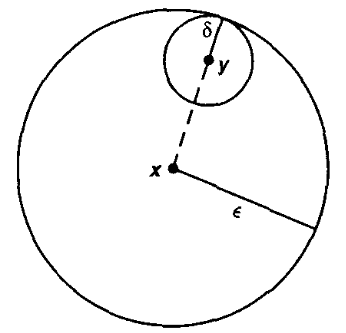
\includegraphics[scale = 0.34]{triangle_inequality_ball_metric.png}}
\end{minipage}
\caption{\footnotesize{\textbf{ $B(y, \delta) \subset B(x, \epsilon)$ for $y \in B(x, \epsilon)$ due to triangle inequality. \citep{munkres2000topology}}}}
\label{fig: triangle_inequality_ball_metric}
\end{figure}


\item \begin{remark} (\emph{\textbf{The Triangle Inequality is Necessary for Basis}})\\
\underline{\emph{\textbf{The triangle inequality conditon}}} is a necessary condition for the $\epsilon$-balls to form a \emph{basis}. It guarantees that for any $y \in B(x, \epsilon)$, there exists a neighborhood of $y$, $B(y, \delta)$ such that $B(y, \delta) \subset B(x, \epsilon)$.

\begin{definition} (\emph{\textbf{Open Set in Metric Topology}})\\
A set $U$ is \emph{\textbf{open}} \emph{in the metric topology} induced by $d$ if and only if for each $y \in U$, there is a $\delta > 0$ such that $B_d(y, \delta) \subset U$.
\end{definition}
\end{remark}

\item \begin{remark} (\emph{\textbf{Other ``Metric-Like" Functions}})\\
Among all algebraic properties that define a metric, \emph{\textbf{the triangle inequality is the strongest}}. There are many ``\emph{metric-like}" functions that do not satisfy the triangle inquality. 
\begin{enumerate}
\item \emph{\textbf{divergence function}}: $D = \divg{}{\cdot}{\cdot}: M \times M  \rightarrow  \bR_{+}$ satisfying for any $p,q \in M$
\begin{align*}
\divg{}{p}{q} > 0,  \text{ and }  \divg{}{p}{q} = 0, \; \text{ iff }p=q.
\end{align*} 
Divergence function \emph{\textbf{does not satiesfy}} neither \emph{the \textbf{symmetric} property} nor \emph{the \textbf{triangle inequality} property}. But it satisfies \emph{the \textbf{positive definiteness} property}. A divergence can act like \emph{\textbf{a measure of closeness} between two points}.

\item \textit{\textbf{inner product}}: for \emph{a vector space $M$}, $\inn{\cdot}{\cdot}: M \times M \rightarrow \bR_{+}$ is a \emph{\textbf{bilinear form}} that \emph{\textbf{satiesfies}} both  \emph{the \textbf{symmetric} property} and \emph{the \textbf{positive definiteness} property}. This makes it \emph{almost a metric}. In fact, \emph{every inner product can induce a \emph{norm} $\norm{x}{} = \sqrt{\inn{x}{x}}$} and thus it can induce a metric via norm $\norm{x - y}{}$

\item \emph{\textbf{semi-norm}}: for \emph{a vector space $M$}, a semi-norm $q: M\rightarrow \bR_{+}$ is a mapping that \emph{\textbf{satiesfies}} both  \emph{the \textbf{homogeneity} property} and \emph{the \textbf{triangle inequality} property}. But it does not satisfies \emph{\textbf{the positive definiteness condition}}. $q(x - y)$ is thus not a metric. It can also be used to \emph{measure the closeness} between two points but \emph{lack of power to tell if these two points are the same}.
\end{enumerate}
\end{remark}

\item \begin{remark} (\emph{\textbf{Metric Topology is Quantitative}})\\
A \emph{\textbf{metric}}  provides a  measurement on the \emph{\textbf{closeness}} between two points. \emph{\textbf{The metric topology}} generated by open balls thus provides a \emph{\textbf{\underline{quantitative descripition} of the neighborhood}} and it answers the question ``\emph{how close the neighborhood of $x$ is} ?" On the other hand, \emph{\textbf{the general topology}} answer this question using \emph{\textbf{\underline{qualitative description}}} via \emph{\textbf{comparison}} with other neighborhoods via the \emph{inclusion} operation $\subset$. Note that inclusion $\subset$ is \emph{\textbf{partially ordered}}, while the metric maps onto the real line where $<$ is \emph{\textbf{simply ordered}}.

\emph{The study of \textbf{topology}} is to acknowledge that \emph{in many areas of research, \textbf{there might not exist a properly defined metric} in the set of interest}. On the other hand, \emph{the study of \textbf{analysis}} mainly focus on \emph{the space equipped with metric topology}.
\end{remark}

\item \begin{definition} (\textbf{\emph{Metrizability}})\\
If $X$ is a topological space, $X$ is said to be \underline{\emph{\textbf{metrizable}}} if \emph{there exists a metric} $d$ on the set $X$ that \emph{induces the topology} of $X$. \underline{\emph{\textbf{A metric space}}} is \emph{a metrizable space} $X$ together with a specific metric $d$ that \emph{gives the topology of $X$}.
\end{definition}

\item \begin{remark} (\emph{\textbf{Metrizability as Inverse Problem}})\\
Given a \emph{metric} $d$ on $X$, we can generate \emph{a metric topology} using $\epsilon$-balls as basis. \emph{\textbf{Conversely}}, \underline{\emph{\textbf{given a topology} $\srT$ on $X$}, \emph{\textbf{is $\srT$ a metric topology for some unknown metric $d$ ?}}} 

This is the question that \emph{\textbf{the metrization theory}} is trying to answer.
\end{remark}

\item \begin{remark} (\emph{\textbf{Metrizability is Valuable}})\\
Many of the spaces important for mathematics are metrizable, but some are not. \emph{\textbf{Metrizability}} is always a highly desirable attribute for a space to possess, for the  existence of a \emph{metric} gives one \emph{a valuable tool} for \emph{proving theorems} about the space.
\end{remark}

\item \begin{definition}
Let $X$ be a metric space with metric $d$. A subset $A$ of $X$ is said to be \emph{\textbf{bounded}} if there is some number $M$ such that
\begin{align*}
d(a_1, a_2) \le M
\end{align*} for every pair $a_1, a_2$ of points of $A$. If $A$ is bounded and nonempty, the \emph{\textbf{diameter}} of $A$ is defined to be the number
\begin{align*}
\text{diam }A = \sup\set{d(a_1, a_2): \forall a_1, a_2 \in A}.
\end{align*}
\end{definition}

\item \begin{remark}
The boundedness property depends on specific metric topology, thus it is not a topological property. 

For instance, the following metric  guarantee that every open set is bounded.
\begin{definition} (\emph{\textbf{Standard Bounded Metric}}) \\
Let $X$ be a metric space with metric $d$. Define $\bar{d} : X \times X \rightarrow \bR$ by the equation
\begin{align*}
\bar{d}(x, y) =\min\{d(x, y), 1\}.
\end{align*}
Then $\bar{d}$ is a \emph{metric} that induces \emph{\textbf{the same topology}} as $d$. 

The metric $\bar{d}$ is called \underline{\emph{\textbf{the standard bounded metric}}} \emph{corresponding to} $d$.
\end{definition}
\end{remark}

\item \begin{definition} (\emph{\textbf{Euclidean Metric and Square Metric}})\\
Given $x = (x_1 \xdotx{,} x_n)$ in $\bR^n$, we define the \emph{\textbf{norm}} of $x$ by the equation
\begin{align*}
\norm{x}{2} &= \paren{x_1^2 \xdotx{+} x_n^2}^{1/2};
\end{align*}
and we define \underline{\emph{\textbf{the euclidean metric}}} $d$ on $\bR^n$ by the equation
\begin{align*}
d(x, y) = \norm{x - y}{2} &= \paren{(x_1 - y_1)^2 \xdotx{+} (x_n - y_n)^2}^{1/2}.
\end{align*}
We define \underline{\emph{\textbf{the square metric}}} $\rho$ by the equation
\begin{align*}
\rho(x, y) &= \max\set{\abs{x_1 - y_1} \xdotx{,} \abs{x_n - y_n}}.
\end{align*}
\end{definition}

\item \begin{lemma}
Let $d$ and $d'$ be two metrics on the set $X$; let $\srT$ and $\srT'$ be the topologies they induce, respectively. Then $\srT'$ is \textbf{finer} than $\srT$ if and only if for each $x$ in $X$ and each $\epsilon > 0$, there exists a $\delta > 0$ such that
\begin{align*}
B_{d'}(x, \delta) \subseteq  B_{d}(x, \epsilon).
\end{align*}
\end{lemma}

\item \begin{proposition}
The topologies on $\bR^n$ induced by \textbf{the euclidean metric} $d$ and \textbf{the square metric} $\rho$ are the \textbf{same} as the \textbf{product topology} on $\bR^n$.
\end{proposition}

\item \begin{remark} (\emph{\textbf{\underline{Finite Dimensional} Vector Space has Only One Meaningful Topology}})\\
In \emph{\textbf{finite dimensional}} vector space, \emph{\textbf{all norms are equivalent}}, and  \emph{all norm-induced metric topologies} are \emph{the same}. For infinite dimenisonal space, these topologies are different.
\end{remark}

\item \begin{definition}(\emph{\textbf{Uniform Topology on Infinite Dimensional Space}})\\
Given an index set $J$, and given points $x = (x_{\alpha})_{\alpha \in J}$ and $y = (y_{\alpha})_{\alpha \in J}$ of $\bR^{J}$, let us define a metric $\bar{\rho}$ on $\bR^{J}$ by the equation
\begin{align*}
\bar{\rho}(x, y) &= \sup\set{\bar{d}(x_{\alpha}, y_{\alpha}): \alpha \in J},
\end{align*}
where $\bar{d}$ is \emph{\textbf{the standard bounded metric}} on $\bR$, It is easy to check that $\bar{p}$ is indeed a metric; it is called \emph{\underline{\textbf{the uniform metric}} on $\bR^{J}$}, and the topology it induces is called \underline{\emph{\textbf{the uniform topology}}}.
\end{definition}

\item \begin{proposition}
The \textbf{uniform topology} on $\bR^{J}$ is \textbf{finer} than the product topology and \textbf{coarser} than the box topology; these three topologies are all different if $J$ is infinite.
\begin{align*}
\srT_{\textbf{product}} \subset \srT_{\textbf{uniform}} \subset \srT_{\textbf{box}}
\end{align*}
\end{proposition}

\item \begin{theorem} (\textbf{Countable Product Space with Product Topology is Metrizable}). \citep{munkres2000topology}\\
Let $\bar{d}(a, b) = \min\set{\abs{a - b},  1}$ be the \textbf{standard bounded metric} on $\bR$. If $x$ and $y$ are two points of $W"$, define
\begin{align*}
D(x, y) &= \sup\set{\frac{\bar{d}(x_i, y_i)}{i}}
\end{align*}
Then $D$ is a metric that induces \textbf{the product topology} on $\bR^{\omega}$.
\end{theorem}
\end{itemize}

\subsubsection{Constructing Continuous Functions on Metric Space}
\begin{itemize}
\item The followings are some important facts about the metric topology:
\begin{enumerate}
\item \begin{proposition}
Every \textbf{metric space $(X, d)$} is \textbf{Hausdorff}.
\end{proposition}

\item \begin{proposition}
Every \textbf{subspace} of metric space $(X, d)$ is a metric space. That is, if $A$ is a subspace of the topological space $X$ and $d$ is a metric for $X$, then the restriction of $d$ on $A \times A$ is a metric for the topology of  $A$.
\end{proposition}
\end{enumerate}


\item \begin{theorem} (\textbf{$\epsilon$-$\delta$ Definition of Continuous Function in Metric Space}). \citep{munkres2000topology} \\
Lei $f: X \rightarrow Y$; let $X$ and $Y$ be \textbf{metrizable} with metrics $d_x$ and $d_y$, respectively. Then \textbf{continuity} of $f$ is \textbf{equivalent} to the requirement that given $x \in X$ and given $\epsilon > 0$, there exists $\delta > 0$ such that
\begin{align*}
d_x(x, y) < \delta \Rightarrow d_{y}(f(x), f(y)) < \epsilon.
\end{align*}
\end{theorem}

\item \begin{remark}
The $\epsilon$-$\delta$ definition of continuous function is equivalent to 
\begin{align*}
f(B(x, \delta)) \subset B(f(x), \epsilon) \quad \Leftrightarrow \quad B(x, \delta) \subset f^{-1}(B(f(x), \epsilon))
\end{align*}
\end{remark}

\item \begin{remark}
To use $\epsilon$-$\delta$ definition, \emph{both \textbf{domain} and \textbf{codomain}} need to be \emph{\textbf{metrizable}}.
\end{remark}

\item \begin{lemma}(\textbf{The Sequence Lemma}). \citep{munkres2000topology}\\
Let $X$ be a topologicaJ space; let $A \subseteq X$. If there is a sequence of points of $A$ \textbf{converging} to $x$, then $x \in \bar{A}$; the \textbf{converse} holds if $X$ is \textbf{metrizable}.
\end{lemma}

\item \begin{proposition}
Let $f: X \rightarrow Y$. If the function $f$ is \textbf{continuous}, then for every \textbf{convergent} sequence $x_n \rightarrow x$ in $X$, the sequence $f(x_n)$ \textbf{converges} to $f(x)$. The \textbf{converse} holds if $X$ is \textbf{metrizable}.
\end{proposition}

\item \begin{remark}
To show the converse part, i.e. ``\emph{if $x_n \rightarrow x \Rightarrow f(x_n) \rightarrow f(x)$ then $f$ is continuous}", we just need the space $X$ to be \emph{\textbf{first countable}}. That is, at each point $x$, there is \emph{\textbf{a countable collection}} $(U_{n})_{n \in \bZ_{+}}$ of \emph{\textbf{neighborhoods}} of $x$ such that any neighborhood $U$ of $x$ \emph{contains} at least one of the sets $U_n$.
\end{remark}

\item \begin{proposition} (\textbf{Arithmetic Operations of Continuous Functions}).\\
If $X$ is a topological space, and if $f, g : X \rightarrow Y$ are continuous functions, then $f + g$,  $f - g$, and $f \cdot g$ are continuous. If $g(x) \neq 0$ for all $x$, then $f/g$ is continuous.
\end{proposition}

\item \begin{definition} (\emph{\textbf{Uniform Convergence}})\\
Let $f_n : X \rightarrow Y$ be a sequence of functions from the \textbf{\emph{set}} $X$ to \emph{\textbf{the metric space}} $Y$. Let $d$ be the metric for $Y$. We say that the sequence $(f_n)$ \underline{\emph{\textbf{converges uniformly}}} to the function $f: X \rightarrow Y$ if given $\epsilon > 0$, there exists an integer $N$ such that
\begin{align*}
d(f_n(x), f(x)) < \epsilon
\end{align*}
for all $n > N$ and \textbf{\emph{all $x$ in $X$}}.
\end{definition}

\item \begin{theorem} (\textbf{Uniform Limit Theorem}). \citep{munkres2000topology}\\
Let $f_n : X \rightarrow Y$ be a sequence of  \textbf{continuous} functions from the \textbf{topological} space $X$ to the \textbf{metric space} $Y$. If $(f_n)$ converges
\textbf{uniformly} to $f$, then $f$ is \textbf{continuous}.
\end{theorem}

\item \begin{remark} (\emph{\textbf{Uniform Convergence $=$ Convergence of Functions in Uniform Metric}})\\
A sequence of functions $f_n : X \rightarrow \bR$ \emph{\textbf{converges uniformly}} to $f: X \rightarrow \bR$ \emph{\textbf{if and only if}} the sequence $(f_n)$ converges to $f$ when they are considered as elements of the metric space $(\bR^{X}, \bar{\rho})$, where $\bR^{X}$ is the space of all real-valued functions on $X$ and $\bar{\rho}$ is \emph{\textbf{the unform metric}} defined before.
\end{remark}

\item \begin{example} 
The \emph{\textbf{countable product space}} $\bR^{\omega}$ in the \emph{\textbf{box topology}} is \emph{\textbf{not metrizable}}. (on the other hand,  it is metrizable \emph{in product topology}).
\end{example}

\item \begin{example}
An \emph{\textbf{uncountable product}} of $\bR$ with itself is \emph{\textbf{not metrizable}}.
\end{example}
\end{itemize}

\subsection{The Quotient Topology}
\subsubsection{Definitions and Properties}
\begin{itemize}
\item \begin{remark} (\emph{\textbf{Quotient Topology as ``Cut-and-Paste"}})\\
One motivation of \emph{\textbf{quotient topology}} comes from geometry, where one often has occasion to use ``\emph{\textbf{cut-and-paste}}" techniques to construct such geometric objects as surfaces.:
\begin{enumerate}
\item The \emph{\textbf{torus}} (surface of a doughnut), for example, can be constructed by taking a \emph{\textbf{rectangle}} and ``\emph{pasting}" its edges together appropriately
\item The \emph{\textbf{sphere}} (surface of a ball) can be constructed by taking a \emph{\textbf{disc}} and \emph{collapsing} its entire boundary to a single point;  
\end{enumerate}
See Figure \ref{fig: quotient_topology}.
\end{remark}


\begin{figure}
\begin{minipage}[t]{1\linewidth}
  \centering
  \centerline{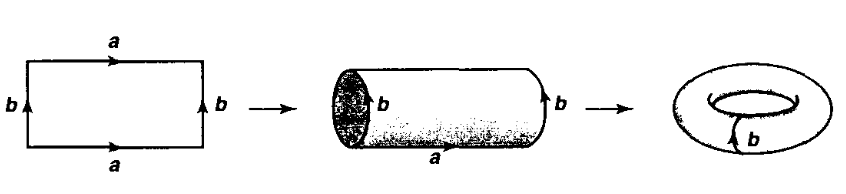
\includegraphics[scale = 0.4]{torus_quotient.png}}
\end{minipage}\\
\begin{minipage}[t]{1\linewidth}
  \centering
  \centerline{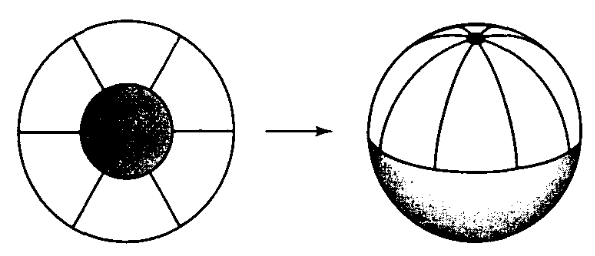
\includegraphics[scale = 0.4]{sphere_quotient.png}}
\end{minipage}
\caption{\footnotesize{\textbf{(Upper) The torus can be constructed via cut-and-paste along the rectangle edges. (Lower) The sphere can be constructed via by taking a disc and collapsing its entire boundary to a single point. \citep{munkres2000topology}}}}
\label{fig: quotient_topology}
\end{figure}


\item \begin{definition} (\emph{\textbf{Quotient Map}})\\
Let $X$ and $Y$ be topological spaces; let $\pi : X \rightarrow Y$ be a \emph{\textbf{surjective map}}. The map $\pi$ is said to be \underline{\emph{\textbf{a quotient map}}} provided a subset $U$ of $Y$ is \emph{\textbf{open}} in $Y$ \underline{\emph{\textbf{if and only if}}} $\pi^{-1}(U)$ is \emph{\textbf{open}} in $X$.
\end{definition}

\item \begin{remark}(\emph{\textbf{Quotient Map $=$ Strong Continuity}})\\
The condition of quotient map is \emph{\textbf{stronger}} than continuity (it is called \underline{\emph{\textbf{strong continuity}}} in some literature). 
\begin{align*}
\text{continuity}: \quad U \text{ is open in }Y & \Rightarrow \pi^{-1}(U) \text{ is open in }X\\
\text{quotient map}: \quad U \text{ is open in }Y & \Leftrightarrow \pi^{-1}(U) \text{ is open in }X
\end{align*}
\emph{An equivalent condition} is to require that a subset $A$ of K be \emph{\textbf{closed}} in $Y$ \emph{if and only if} $\pi^{-1}(A)$ is \emph{\textbf{closed}} in $X$. Equivalence of the two conditions follows from equation
\begin{align*}
\pi^{-1}(Y \setminus B) = X \setminus \pi^{-1}(B).
\end{align*}
\end{remark}

\item \begin{definition} (\emph{\textbf{Saturated Set and Fiber}})\\
If $\pi: X \rightarrow Y$ is a \emph{\textbf{surjective} map}, a subset $U \subseteq X$ is said to be \underline{\emph{\textbf{saturated}}} with respect to $\pi$ if $U$ contains every set $\pi^{-1}(\{y\})$ that it \emph{\textbf{intersects}}. Thus $U$ is \emph{\textbf{saturated}} if it equals to the \textbf{\emph{entire preimage}} of its \emph{\textbf{image}}: $U =\pi^{-1}(\pi(U))$. 

Given $y \in Y$, the \underline{\emph{\textbf{fiber}}} of $\pi$ over $y$ is the set $\pi^{-1}(\{y\})$. 
\end{definition}

\item \begin{definition} (\emph{\textbf{Quotient Map via Saturated Set}})\\
A surjective map $\pi : X \rightarrow Y$ is a \underline{\emph{\textbf{quotient map}}} if $\pi$ is \emph{\textbf{continuous}} and $\pi$ maps \emph{\textbf{saturated open sets}} of $X$ to \emph{\textbf{open sets}} of $Y$ (or \emph{saturated closed sets} of $X$ to \emph{closed sets} of $Y$).
\end{definition}


\item \begin{definition} (\emph{\textbf{Open Map} and \textbf{Closed Map}})\\
A map $f: X \rightarrow Y$ (continuous or not) is said to be an \underline{\emph{\textbf{open map}}} if for every \emph{open} subset $U \subseteq X$, the image set $f(U)$ is \emph{open} in $Y$, and a  \underline{\emph{\textbf{closed map}}} if for every \emph{closed} subset $K \subseteq X$, the image $f(K)$ is \emph{closed} in Y . 
\end{definition}

\item \begin{proposition}
If $\pi: X \rightarrow Y$ is a \textbf{surjective continuous} map that is \textbf{either} \textbf{open} or \textbf{closed}, then $\pi$ is a \textbf{quotient} map.
\end{proposition}
\begin{remark}
There are \emph{quotient maps} that are \emph{\textbf{neither}} \emph{open} nor \emph{closed}. See Exercise in \citep{munkres2000topology}.
\end{remark}

\item \begin{example} (\emph{\textbf{Coordinate Projection as Quotient Map}})\\
Let $\pi_1 : \bR \times \bR \rightarrow \bR$ be \emph{\textbf{projection onto the first coordinate}}; then $\pi_1$ is \emph{continuous} and \emph{surjective}. Furthermore, $\pi_1$ is an \underline{\emph{\textbf{open map}}}. For if $U \times V$ is a nonempty \emph{basis element} for $\bR \times \bR$, then $\pi_1(U \times V) = U$ is \emph{open} in $\bR$; it follows that $\pi_1$ carries open sets of $\bR \times \bR$ to open sets of $\bR$. That is, $\pi_1$ is a \emph{\textbf{quotient map}}.

However, $\pi_1$ is \emph{\textbf{not} a \textbf{closed map}}. The subset
\begin{align*}
C = \set{(x, y): x \cdot y =1}
\end{align*}
of $\bR \times \bR$ is \emph{closed}, but $\pi_1(C) = \bR \setminus \{0\}$, which is \emph{not closed} in $\bR$.
\end{example}

\item \begin{definition} (\emph{\textbf{Quotient Topology}})\\
If $X$ is a space and $A$ is a set and if $\pi: X \rightarrow A$ is a \textbf{\emph{surjective}} map, then there exists \textbf{\emph{exactly one topology $\srT$ on $A$}} relative to which $\pi$ is a \emph{\textbf{quotient map}}; it is called \underline{\emph{\textbf{the quotient topology}} induced by $\pi$}. \emph{The quotient topology} $\srT$ on $A$ is defined as
\begin{align*}
\srT = \set{U \subset A:  \pi^{-1}(U) \text{\emph{ is open in }} X}
\end{align*}
\end{definition}



\item \begin{definition}(\emph{\textbf{Quotient Space}})\\
Suppose $X$ is a topological space and $\sim$ is \emph{an equivalence relation} on $X$. Let $X/\sim$ denote \emph{\textbf{the set of equivalence classes}} in $X$, and let $\pi: X \rightarrow X/\sim$ be the \emph{\textbf{natural projection}} sending each \emph{point} to its \emph{equivalence class}. Endowed with \emph{\textbf{the quotient topology}} determined by $\pi$, the space $X/\sim$ is called \underline{\emph{\textbf{the quotient space}}} (or \emph{identification space}) of $X$ determined by $\pi$.
\end{definition}

\begin{definition} \citep{munkres2000topology}\\
Let $X$ be a topological space, and let $X^{*}$ be a \emph{\textbf{partition}} of $X$ into \emph{disjoint subsets whose union is $X$}. Let $\pi: X \rightarrow X^*$ be the \emph{\textbf{surjective}} map that carries each point of $X$ to the element of $X^*$ \emph{containing} it. In \emph{\textbf{the quotient topology}} induced by $\pi$, the space $X^*$ is called a \emph{\textbf{quotient space} of $X$}.
\end{definition}

\item \begin{remark} (\emph{\textbf{Understanding Topology of Quotient Space}})\\
We can describe the topology of $X/\sim$ in another way. A \emph{subset} $U$ of $X/\sim$ is \emph{\textbf{a collection of equivalence classes}}, and the set $\pi^{-1}(U)$ is just \emph{\textbf{the union} of \textbf{the equivalence classes belonging to $U$}}. 

Thus the typical \underline{\emph{\textbf{open set}} of $X/\sim$} is \emph{\textbf{a collection} of \textbf{equivalence classes}} whose \underline{\emph{\textbf{union}}} is \underline{\emph{\textbf{an open set}}} of $X$.
\begin{align*}
V \text{ open in } X/\sim \quad &\Leftrightarrow \quad U:=\pi^{-1}(V) = \bigcup_{[y] \in V}\brac{y} \text{ open in } X
\end{align*}
\end{remark}

\item \begin{remark} (\emph{\textbf{Geometrical Understanding of Quotient Space}})\\
\emph{A set of points in $X$ in the \textbf{same equivalence class} $[y]$  is considered as \textbf{one point} in quotient space $X/\sim$}. Geometrically, it is seen as \emph{\textbf{collapsing} \textbf{a set of points} into \textbf{one}} if this set of points are in a connected neighborhood, or, it is seen as \emph{\textbf{cut-and paste} a set of points in boundary} with another set of points in boundary.
\end{remark}

\item \begin{example} ($\mathds{D}^2/\sim =  \bS^2$)\\
Let $X$ be the \emph{\textbf{closed unit ball}}
\begin{align*}
X = \mathds{D}^2 := \set{(x, y): x^2 + y^2 \le 1}
\end{align*}
in $\bR^2$, and let $X/\sim$ be the partition of $X$ consisting of all the one-point sets $\{(x, y)\}$ for
which $x^2 + y^2 < 1$, along with the set $\bS^1 = \{(x,y): x^2 + y^2 = 1\}$. One can show that $X/\sim$ is \emph{homeomorphic} with the subspace of $\bR^3$ called \emph{\textbf{the unit 2-sphere}}, defined by
\begin{align*}
\set{(x, y, z): x^2 + y^2 + z^2 = 1}
\end{align*}
\end{example}


\item \begin{proposition} (\textbf{Restricting Quotient Map to Subspace}). \citep{munkres2000topology}\\
Let $\pi : X \rightarrow Y$ be a \textbf{quotient map}; let $A$ be a subspace of $X$ that is \textbf{saturated} with respect to $\pi$; let $q : A \rightarrow \pi(A)$ be the map obtained by restricting $\pi$.
\begin{enumerate}
\item If $A$ is either \textbf{open} or \textbf{closed} in $X$, then $q$ is a \textbf{quotient map}.
\item If $\pi$ is either an \textbf{open map} or a \textbf{closed map}, then $q$ is a \textbf{quotient map}.
\end{enumerate}
\end{proposition}

\item \begin{remark} (\textbf{\emph{Composite of Quotient Maps is Quotient Map}}). \\
Composites of maps  behave nicely; it is easy to check that the \emph{composite of two quotient maps is a quotient map}; this fact follows from the equation
\begin{align*}
p^{-1}(q^{-1}(U)) &= (q\circ p)^{-1}(U).
\end{align*}
\end{remark}

\item \begin{remark} (\textbf{\emph{Product of Quotient Maps Need Not to be Quotient Map}}). \\
On the other hand, products of maps do not behave well; \emph{the cartesian product of two quotient maps \textbf{need not} be a quotient map}. 

One needs further conditions on either the maps or the spaces in order for this statement to be true. 
\begin{enumerate}
\item One such, a condition on the spaces, is called \emph{\textbf{local compactness}}; we shall study it later. 
\item Another, a condition on the \emph{maps}, is the condition that \emph{\textbf{both} the maps $p$ and $q$ be \textbf{open maps}}. In that case, it is easy to see that $p \times q$ is also \emph{\textbf{an open map}}, so it is a quotient map.
\end{enumerate}
\end{remark}

\item \begin{remark} (\emph{\textbf{Quotient Space of Haudorff Space Need Not to be Hausdorff}})\\
The Hausdorff condition does not behave well; \emph{even if $X$ is Hausdorff, there is no reason that the quotient space $X/\sim$ needs to be Hausdorff}. There is a simple condition for $X/\sim$ to satisfy the $T_1$ axiom; one simply requires that \emph{\textbf{each element} of the partition $X/\sim$ be a \textbf{closed subset} of $X$}. Conditions that will ensure $X/\sim$ is \emph{Hausdorff} are harder to find.
\end{remark}

\end{itemize}
\subsubsection{Constructing Continuous Function on Quotient Space}
\begin{itemize}
\item We want to know if $f: (X/\sim) \rightarrow Z$ is \emph{continuous function}. 

\item \begin{theorem}  (\textbf{Passing Continuity to the Quotient}). \citep{munkres2000topology}\\
Let $\pi: X \rightarrow Y$ be a \textbf{quotient map}. Let $Z$ be a space and let $g : X \rightarrow Z$ be a map that is \textbf{constant} on \textbf{each fiber}  $\pi^{-1}(\{y\})$, for $y \in Y$. Then $g$ \textbf{induces} a map $f: Y \rightarrow Z$ such that $f \circ \pi = g$. The induced map $f$ is \textbf{continuous} if and only
if $g$ is \textbf{continuous}: $f$ is a \textbf{quotient map} if and only if $g$ is a \textbf{quotient map}.
\[
  \begin{tikzcd}
     X  \arrow[swap]{d}{\pi} \arrow[dr, "g"]  & \\
     Y   \arrow[r, swap, dashed,  "f"]  & Z.
  \end{tikzcd}
\] 
\end{theorem}

\item \begin{corollary}
Let $g : X \rightarrow Z$ be a \textbf{surjective continuous} map. Let $X/\sim$ be the following collection of subsets of $X$:
\begin{align*}
X/\sim := \set{g^{-1}(\{z\}): z \in Z },
\end{align*}
Given $X/\sim$ the \textbf{quotient topology},
\begin{enumerate}
\item The map $g$ induces a \textbf{bijective continuous map} $f : (X/\sim) \rightarrow Z$, which is a \textbf{homeomorphism} \textbf{if and only if} $g$ is a \textbf{quotient map}.
\item If $Z$ is \textbf{Hausdorff}, so is $X/\sim$.
\end{enumerate}
\[
  \begin{tikzcd}
     X  \arrow[swap]{d}{\pi} \arrow[dr, "g"]  & \\
     (X/\sim)   \arrow[r, swap, dashed,  "f"]  & Z.
  \end{tikzcd}
\] 
\end{corollary}

\item \begin{example}(\emph{\textbf{The Product of two Quotient Maps Need Not be a Quotient Map}}).\\
Let $X = \bR$ and let $X/\sim$ be the \emph{quotient space} obtained from $X$ by \emph{\textbf{identifying}} the subset $\bZ_{+}$ to a point $b$; let $\pi : X \rightarrow X/\sim$ be the quotient map. Let $\bQ$ be the subspace of $\bR$ consisting of \emph{the rational numbers}; let $i : \bQ \rightarrow \bQ$ be the \emph{identity map}. We show that
\begin{align*}
\pi \times i: X \times \bQ \rightarrow (X/\sim) \times \bQ
\end{align*}
is \emph{\textbf{not a quotient map}}.

For each $n$, let $c_n = \sqrt{2}/n$, and consider \emph{the straight lines} in $\bR^2$ with slopes $1$ and $-1$, respectively, through the point $(n, c_n)$. Let $U_n$ consist of \emph{all points of $X \times \bQ$ that lie \textbf{above both} of these lines \textbf{or beneath both} of them}, and also \emph{between the vertical lines $x = n - 1/4$ and $x = n + 1/4$}. Then $U_{n}$ is \emph{\textbf{open}} in $X \times \bQ$; it contains the set $\{n\} \times \bQ$ because $c_{n}$ is \emph{\textbf{not rational}}. 

Let $U$ be the \emph{\textbf{union}} of the sets $U_n$; then $U$ is \emph{\textbf{open}} in $X \times \bQ$. It is \emph{\textbf{saturated}} with respect
to $\pi \times i$ because it \emph{contains the entire set $\bZ_{+} \times \set{q}$) for each $q \in \bQ$}. We assume that $U' := (\pi \times i)(U)$ is \emph{\textbf{open}} in $(X/\sim) \times \bQ$ and derive a \emph{contradiction}.

Because $U$ contains, in particular, the set  $\bZ_{+} \times \set{0}$, the set $U'$ contains the point $(b, 0)$. Hence $U'$ contains an \emph{open set} of the form $W \times I_{\delta}$, where $W$ is a neighborhood of $b$ in $X/\sim$ and $I_{\delta}$ consists of all \emph{rational numbers} $y$ with $\abs{y} < \delta$. Then
\begin{align*}
\pi^{-1}(W) \times I_{\delta} \subset U.
\end{align*}
Choose $n$ large enough that $c_n < \delta$. Then since $\pi^{-1}(W)$ is \emph{open} in $X$ and contains $\bZ_{+}$, we can choose $\epsilon < 1/4$ so that the interval $(n - \epsilon, n + \epsilon)$ is contained in $\pi^{-1}(W)$. Then $U$ contains the subset $V =(n - \epsilon, n + \epsilon) \times  I_{\delta}$ of $X \times \bQ$. But the figure makes clear that there are many points $(x, y)$ of $V$ that do not lie in $U'$. (One such is the point $(x, y)$, where $x = n + \frac{1}{2}\epsilon$ and $y$ is a \textbf{\emph{rational number}} with $\abs{y - c_{n}} < \frac{1}{2}\epsilon$.)

\begin{figure}
\begin{minipage}[t]{1\linewidth}
  \centering
  \centerline{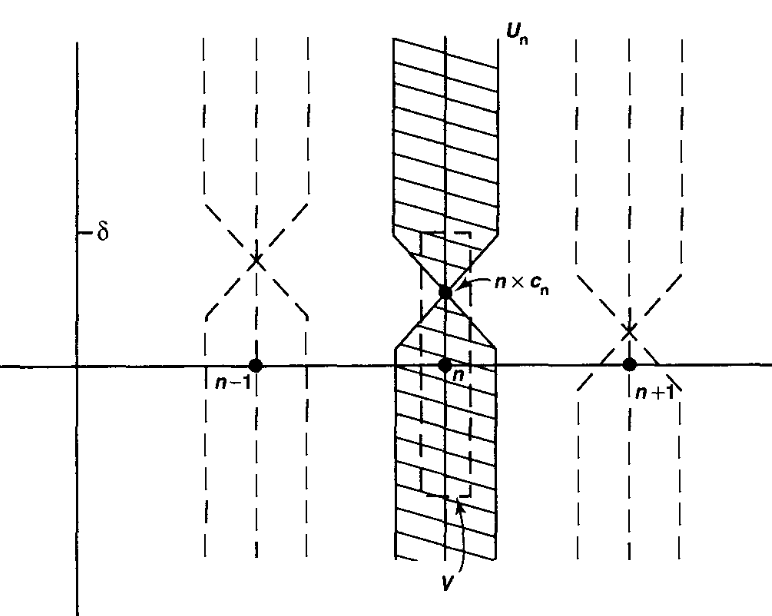
\includegraphics[scale = 0.3]{non_hausdorff_quotient_product.png}}
\end{minipage}
\caption{\footnotesize{\textbf{The product of two quotient maps need not be a quotient map. \citep{munkres2000topology}}}}
\label{fig: non_hausdorff_quotient_product}
\end{figure}
\end{example}
\end{itemize}

\section{Topological Groups}
\begin{itemize}
\item \begin{definition} (\emph{\textbf{Topological Group}})\\
A \underline{\emph{\textbf{topological group}}} $G$ is a \emph{\textbf{group}} that is also a \emph{\textbf{topological space}} satisfying \emph{\textbf{the $T_1$ axiom}}, such that  \emph{\textbf{the multiplication map}} $m: G \times G \rightarrow G$ and \emph{\textbf{inversion map}} $i: G \rightarrow G$, given by
\begin{align*}
m(x, y) = x y, \quad i(x) = x^{-1}.
\end{align*} are both \emph{\textbf{continuous maps}}. Here, $G\times G$ is viewed as a \emph{topological space} by using \emph{the product topology}.
\end{definition}

\item \begin{example} (\emph{\textbf{Common Topological Groups}})\\
The following are topological groups:
\begin{enumerate}
\item $(\bZ, +)$
\item $(\bR, +)$
\item $(\bR_{+}, \cdot)$
\item $(\bS^1, \cdot)$, where we take $\bS^1$ to be \emph{the space of \textbf{all complex numbers} $z$} for which $\abs{z} = 1$
\end{enumerate}
\end{example}

\item \begin{example} (\emph{\textbf{Lie Groups}})
\begin{definition} (\emph{\textbf{Lie Group}}) \citep{lee2003introduction}\\
A \underline{\emph{\textbf{Lie group}}} is a \emph{\textbf{smooth manifold}} $\cG$ (without boundary) that is also \emph{a \textbf{group}} in the
\emph{algebraic sense}, with the property that \emph{the multiplication map} $m: G \times G \rightarrow G$ and \emph{inversion map} $i: G \rightarrow G$, given by
\begin{align*}
m(g, h) = g h, \quad i(g) = g^{-1}.
\end{align*} are both \emph{\textbf{smooth}}. 
\end{definition}
\underline{\emph{\textbf{A Lie group is a topological group}}}. The followings are all \emph{\textbf{Lie groups}}:
\begin{enumerate}
\item \underline{\emph{\textbf{The general linear group}}} $GL(n, \bR)$ is the set of \emph{\textbf{invertible} $n\times n$ matrices} with real entries.
\begin{align*}
GL(n, \bR) &\equiv \set{\mb{A}\in \bR^{n\times n}:\; \det\paren{\mb{A}}\neq 0}. 
\end{align*}
It is a \emph{group} under \emph{\textbf{matrix multiplication}}, and it is an \emph{open submanifold} of the vector space $M(n, \bR) \simeq \bR^{n \times n}$. \emph{Multiplication is smooth} because \emph{the matrix entries} of a product matrix $AB$ are \emph{polynomials} in the entries of $A$ and $B$. Inversion is \emph{smooth} by \emph{Cramer's rule}.

\item Let $GL_{+}(n, \bR)$  denote the subset of $GL(n, \bR)$ consisting of matrices with \emph{\textbf{positive determinant}}. Because $\det(AB) =\det(A)\det(B)$ and $\det(A^{-1})= (\det(A))^{-1}$, it is a subgroup of $GL(n, \bR)$; and because it is the \emph{preimage} of $(0, +\infty)$ under \emph{the continuous determinant function}, it is an open subset of $GL(n, \bR)$ and therefore an $n^2$-dimensional manifold. The \emph{group operations} are the restrictions of those of $GL(n, \bR)$, so they are smooth. Thus  $GL_{+}(n, \bR)$ is a \emph{Lie group}.

\item The \underline{\emph{\textbf{special linear group}}} $SL(n, \bR)$ is the subgroup of $GL(n, \bR)$ consisting of matrices with a \emph{\textbf{determinant of $1$}}.
\begin{align*}
SL(n, \bR) &\equiv \set{\mb{A}\in \bR^{n\times n}:\; \det\paren{\mb{A}}= 1}. 
\end{align*}
It is a \emph{Lie group} with dimension $\dim{SL(n,\bR)} = n^{2} - 1.$ 

\item The \emph{\underline{\textbf{orthogonal group}} of dimension $n$}, denoted $\mathcal{O}(n)$, is the group of \emph{\textbf{distance-preserving transformations}} of a Euclidean space of dimension $n$ that preserve a fixed point, where the group operation is given by composing transformations. Also, $(\cO(n), \cdot)$ is the group of $n\times n$ \emph{\textbf{orthogonal matrices}}, where the group operation $(\cdot)$ is given by matrix multiplication, and an orthogonal matrix is a real matrix whose inverse equals its transpose. \emph{The orthogonal group is a Lie group} with \emph{dimension} $n(n-1)/2$.
\begin{align*}
\cO(n) &\equiv \set{\mb{Q}\in GL(n, \bR):\;  \mb{Q}^{T}\mb{Q} = \mb{Q}\mb{Q}^{T} = \mb{I}_{n}}.
\end{align*}

\item The \underline{\emph{\textbf{special orthogonal group}}} $\cS\cO(n)$ is the group of \emph{the \textbf{orthogonal matrices} of \textbf{determinant} $1$}. This group is also called the \underline{\emph{\textbf{rotation group}}}
\begin{align*}
\cS\cO(n) &\equiv \set{\mb{Q}\in \cO(n):\;  \det\paren{\mb{Q}}= 1}.
\end{align*} It is an open subgroup of $\cO(n)$, which is a \emph{Lie group} of dimension $\dim{\cS\cO(n)}= \dim{\cO(n)} = n(n-1)/2$.

\item \emph{\textbf{The complex general linear group}} $GL(n, \bC)$ is the group of \emph{invertible complex $n\times n$ matrices} under matrix multiplication. It is an open submanifold of $M(n, \bC)$ and thus a $2n^2$-dimensional smooth manifold, and it is a \emph{Lie group} because \emph{matrix products and inverses} are \emph{smooth functions} of the real and imaginary parts of the matrix entries.

\item If $V$ is any \emph{real or complex vector space}, $GL(V)$ denotes \emph{the set of \textbf{invertible linear maps}} from $V$ to itself. It is a \emph{group under composition}.  If $V$ has \emph{\textbf{finite dimension}} $n$, any basis for $V$ determines an \emph{isomorphism} of $GL(V)$ with $GL(n, \bR)$  or $GL(n, \bC)$, so $GL(V)$ is a \emph{Lie group}. 

\item $(\bZ, +)$
\item $(\bR, +)$
\item The set $\bR^{*}$ of \emph{nonzero real numbers} is a \emph{\textbf{$1$-dimensional Lie group} under multiplication}. (In fact, it is exactly $GL(1, \bR)$ if we identify a $1\times 1$ matrix with the corresponding real number.) The subset $\bR_{+}$ of \emph{\textbf{positive real numbers}} is an \emph{open subgroup}, and is thus itself a \emph{$1$-dimensional Lie group}.
\item The set $\bC^{*}$ of \emph{\textbf{nonzero complex numbers}} is a \emph{$2$-dimensional} \emph{Lie group} under complex multiplication, which can be identified with $GL(1, \bC)$.
\item  The \emph{\textbf{circle}} $\bS^1\subset \bC^{*}$ is a smooth manifold and a group under complex multiplication. With appropriate \emph{\textbf{angle functions}} as \emph{local coordinates} on open subsets of $\bS^1$, \emph{multiplication and inversion} have the \emph{smooth coordinate expressions} $(\theta_1, \theta_2) \mapsto \theta_1 + \theta_2$ and $\theta \mapsto -theta$, and therefore $\bS^1$ is a Lie group, called \underline{\emph{\textbf{the circle group}}}.
\item The \underline{\emph{\textbf{$n$-torus}}} $\bT^n = \bS^1 \xdotx{\times} \bS^1$ is an \emph{\textbf{$n$-dimensional abelian Lie group}}.
\end{enumerate}
\end{example}

\item \begin{example} (\emph{\textbf{Discrete Group}})\\
Any \emph{\textbf{group}} with \emph{\textbf{the discrete topology}} is a \emph{topological group}, called a \underline{\emph{\textbf{discrete group}}}. If in addition the group is \emph{finite} or \emph{countably infinite}, then it is a \emph{\textbf{zero-dimensional Lie group}}, called a \underline{\emph{\textbf{discrete Lie group}}}.
\end{example}

\item \begin{definition} (\emph{\textbf{Homogeneous Space}})\\
A topological space $G$ is a \underline{\emph{\textbf{homogeneous space}}} if for every pair $x,y\in G$, there exists a \emph{homemorphism} $f: G\to G$ such that $f(x) = y$. 
\end{definition}

\item \begin{proposition} (\textbf{Topological Groups Are Homogeneous})\\
Every \textbf{topological group} is a \textbf{homogeneous} space; in particular, define map $h_{\alpha}: G\to G$ as $h_{\alpha}(x) = \alpha\cdot x$ and $g_{\alpha}: G\to G$ as $g_{\alpha}(x) = x \cdot \alpha$, for $\alpha\in G$. Then $h_{\alpha}, \, g_{\alpha}$ are \textbf{homemorphisms}.
\end{proposition}

\item \begin{proposition} (\textbf{Subgroup of Topological Group})\\
Let $H$ be a \textbf{subspace} of topological group $G$. If $H$ is also a \textbf{subgroup} of G, then both $H$ and its closure $\bar{H}$ are \textbf{topological groups}.
\end{proposition}

\item \begin{definition} (\emph{\textbf{Left Coset} and \textbf{Right Coset}})\\
For $H\subset G$ as the \emph{subgroup} of $G$, define the \underline{\emph{\textbf{left coset}}} as $xH = \set{x\cdot h: h\in H}$. Similarly, define \underline{\emph{\textbf{the right coset}}} as $Hx = \set{h\cdot x: h\in H}$
\end{definition}

\item \begin{definition} (\emph{\textbf{Quotient Group}})\\
The collection of \emph{left cosets} defines a \underline{\emph{\textbf{quotient group}}} $G/H = \set{ xH\, |\, x\in G}$ with \emph{the group operation} $xH \cdot yH = (x\cdot y) H$.  
\end{definition}

\item \begin{proposition}
Let $G$ be a topological group.
\begin{enumerate}
\item If $\alpha \in G$, the map $f_\alpha: x \mapsto \alpha \cdot x$  induces a homeomorphism of $G/H$ carrying $xH$ to $(\alpha \cdot x)H$. Thus  $G/H$ is a \textbf{homogeneous space}.
\item If $H$ is a \textbf{closed} set in the topology of $G$, then \textbf{one-point sets} are \textbf{closed} in $G/H$.
\item The \textbf{quotient map} $\pi: G \rightarrow G/H$ is \textbf{open}.
\item If $H$ is \textbf{closed} in the topology of $G$ and is a \textbf{normal subgroup} of $G$, then the (left) quotient group $G/H$ under quotient topology is a \textbf{topological group}. 
\item If $H$ is \textbf{compact} \textbf{subgroup} of $G$ and $\pi: G \rightarrow G/H$ is closed, then $G/H$ is \textbf{compact}.
\end{enumerate}
\end{proposition}

\item \begin{example} ($GL(n, \bR)/SL(n, \bR) \simeq \bR^{*} = \bR \setminus \set{0}$).\\
Given the \emph{generalized linear group} $GL(n, \bR)$, \emph{the special linear group} $SL(n, \bR)$ is a subgroup of $GL(n, \bR)$. The \emph{quotient group} $GL(n, \bR)/SL(n, \bR) \simeq \bR^{*} = \bR \setminus \set{0}$.
\end{example}
\begin{proof}
Let $G = GL(n, \bR)$ and $H = SL(n, \bR) = \set{\mb{A}\in \bR^{n\times n}:\; \det\paren{\mb{A}}= 1}$.  Define $\det: GL(n, \bR) \rightarrow \bR^{*}$. The map $\det$ is constant on each left coset 
\begin{align*}
xH = (\det{})^{-1}(r);
\end{align*} where $x \in G$ with $\det(x) = r \neq 0$. Note that for all $\mb{A} \in xH$, $\mb{A} = x\mb{S}$ where $\mb{S}$ is the matrix in $SL(n, \bR)$. so $\det(\mb{A}) = \det(x)\det(\mb{S}) = \det(x) = r$ since $\det{\mb{S}} = 1$.  Moreover $\det$ is a \emph{surjective continuous} map. Now we show that $\det$ is an open map, therefore $\det: GL(n, \bR) \rightarrow \bR^{*}$ is a quotient map.

To prove that $\det(\text{any open subset of }GL(n, \bR))$ is an open set in $\bR^{*}$, consider the matrix $\mb{A} \in GL(n, \bR)$, note that by expansion by minor, the determinant of $\mb{A}$ can be written as
\begin{align*}
\det\paren{\mb{A}} &= \sum_{i=1}^{m}(-1)^{i-1}a_{1,i}\det(\mb{A}_{-i})\\
\det\paren{\mb{A}+ \delta \mb{E}_{k}} &= \sum_{i=1}^{m}(-1)^{i-1}(a_{1,i} + \delta\,\mathds{1}_{i,k})\det(\mb{A}_{-i})\\
&= \det\paren{\mb{A}} + (-1)^{k-1} \delta\det(\mb{A}_{-k})\\
\abs{\det\paren{\mb{A}+ \delta \mb{E}_{k}} - \det\paren{\mb{A}}} &\le  \epsilon
\end{align*} 


From the corollary above, there exists a bijective continuous map $f: G/H \rightarrow \bR^{*}$ so that the following diagram commutes
\[
  \begin{tikzcd}
     G  \arrow[swap]{d}{\pi} \arrow[dr, "\det"]  & \\
     (G/H)   \arrow[r, swap, dashed,  "f"]  & \bR^{*} .
  \end{tikzcd}
\]  Since $\det: GL(n, \bR) \rightarrow \bR^{*}$ is a quotient map, $f$ is a \emph{homemorphism}. \qed
\end{proof}

\item \begin{example} ($GL(n, \bR)/SL(n, \bR) \simeq \bR^{*} = \bR \setminus \set{0}$).\\
Given the \emph{generalized linear group} $GL(n, \bR)$, \emph{the special linear group} $SL(n, \bR)$ is a subgroup of $GL(n, \bR)$. The \emph{quotient group} $GL(n, \bR)/SL(n, \bR) \simeq \bR^{*} = \bR \setminus \set{0}$.
\end{example}

\item \begin{example}  ($\cO(n)/\cS\cO(n) \simeq \bZ_{2} =\set{-1, 1} = \bZ / 2\bZ$).\\
The quotient group of orthogonal group $\cO(n)$ over the special orthorognal group $\cS\cO(n) = \set{\mb{Q}\in \cO(n):\;  \det\paren{\mb{Q}}= 1}$ is homemorphic to $\bZ_{2} = \set{-1, 1}$.
\end{example}


\item \begin{example}  ($\cO(n)/\cO(n-1) \simeq \bS^{n-1}$).\\
The quotient group of $n$-dimensional orthogonal group $\cO(n)$ over $(n-1)$-dimensional orthogonal group $\cO(n-1)$  is homemorphic to $(n-1)$-dimensional sphere $\bS^{n-1}$.
\end{example}

\item \begin{definition} (\emph{\textbf{Topological Group Action}})\\
An \underline{\emph{\textbf{action}}} of a \emph{\textbf{topological group}} $G$ on a \emph{\textbf{topological space}} $X$ is a \emph{\textbf{continuous map}} $\phi: G \times X \rightarrow X$ such that for $g(x):= \phi(g, x)$, 
\begin{align*}
(g_1 \cdot g_2)(x)  &= g_1(g_2(x)), && \quad \forall g_1, g_2 \in G, x\in X\\
1_{G}(x) &= \text{Id}_{X}(x) = x, &&\quad \forall x\in X
\end{align*} where $1_{G}$ is the unit element of group $G$. Together with the group action, $X$ is called a \underline{\emph{\textbf{$G$-space}}}.
\end{definition}

\item \begin{remark}
The map $x \mapsto g(x)$ is a \emph{\textbf{continuous map}} on $X$ for each $g\in G$. This map has \emph{\textbf{inverse map}} $x \mapsto g^{-1}(x)$ which is continuous as well. Thus the map $x \mapsto g(x)$ is a \underline{\emph{\textbf{homemorphism}}}.
\end{remark}

\item \begin{example}
\emph{The topological group} $\cO(n)$ \emph{acts} on $\bR^n$ is the rotation transformation of vectors in $\bR^n$. Similarly, $\cO(n)$ \emph{acts} on $\bS^1$ is the rotation of circle $\bS^1$.
\end{example}

\item \begin{definition}(\emph{\textbf{Orbit under Topological Group Actions}})\\
If \emph{the topological group} $G$ \emph{acts} on topological space $X$, and $x \in X$, then \underline{\emph{\textbf{the orbit} of $x$}} is defined as
\begin{align*}
G(x) &= \set{g(x): g\in G}
\end{align*}
\end{definition}

\item \begin{definition}
The \emph{\textbf{stablizer}} of $x$ under group actions $G$ is defined as 
\begin{align*}
G_x = \set{g\in G: g(x) = x}
\end{align*}
\end{definition}

\item \begin{definition} (\emph{\textbf{Orbit Space $X/G$}})\\
Let $G$ be a topological group and $X$ be a \emph{$G$-space} so that $G$ acts on $X$. \underline{\emph{\textbf{The orbit space}}} is the set of \emph{all orbits of action} with \emph{quotient topology}. The quotient map $\pi: x \mapsto G(x)$ maps $x$ to its orbit. \emph{The orbit space} is often called \underline{\emph{\textbf{the quotient of $X$ by group actions $G$}}}, i.e. 
\begin{align*}
X/G &= \set{G(x): x \in X}.
\end{align*}
\end{definition}

\item \begin{proposition} (\textbf{Orbit Space by Compact Group})\\
Let $G$ be a \textbf{compact} topological group and $X$ be a topological space so that $G$ acts on $X$. Let $X/G$ be the \textbf{orbit space}, i.e. the quotient space of $X$ by group actions $G$. Then
\begin{enumerate}
\item $X/G$ is \textbf{Hausdorff} if $X$ is \textbf{Hausdorff};
\item $X/G$ is \textbf{regular} if $X$ is \textbf{regular};
\item $X/G$ is \textbf{normal} if $X$ is \textbf{normal};
\item $X/G$ is \textbf{locally compact} if $X$ is \textbf{locally compact};
\item $X/G$ is \textbf{second countable} if $X$ is \textbf{second countable};
\end{enumerate}
\end{proposition}

\item \begin{example}(\emph{\textbf{Global Flow on Smooth Manifold}}) \citep{lee2003introduction}
 \begin{definition}
A \underline{\emph{\textbf{global flow on $M$}}} (also called \textbf{\emph{a one-parameter group action}}) is defined as a \emph{\textbf{continuous left $\bR$-action on $M$}}; that is, a \emph{continuous map} $\theta:  \bR \times M \rightarrow M$ satisfying the following properties for all $s, t \in \bR$ and $p \in M$:
\begin{align*}
\theta_{t+s}(p) &= \theta_t \circ \theta_s(p), \\
\theta_0(p)&= p 
\end{align*} where $\theta_t = \theta(t, \cdot): M \rightarrow M$ is a \emph{continuous map} and $\theta_0 = \text{Id}_{M}$. 
\end{definition}
As we can see that, \emph{\textbf{the global flow is topological group action} of $(\bR, +)$ on the smooth manifold $M$ (a topological space)}.

 \begin{definition}
For each $p \in M$, define a curve $\theta^{(p)}: \bR \rightarrow M$ by
\begin{align*}
\theta^{(p)}(t) &= \theta(t, p).
\end{align*} The image of this curve is \emph{\textbf{the \underline{orbit} of $p$ under the group action}}.
\end{definition}
\end{example}
\end{itemize}


\newpage
\bibliographystyle{plainnat}
\bibliography{book_reference.bib}
\end{document}